% Options for packages loaded elsewhere
\PassOptionsToPackage{unicode}{hyperref}
\PassOptionsToPackage{hyphens}{url}
%
\documentclass[
  11pt,
]{article}
\usepackage{lmodern}
\usepackage{amssymb,amsmath}
\usepackage{ifxetex,ifluatex}
\ifnum 0\ifxetex 1\fi\ifluatex 1\fi=0 % if pdftex
  \usepackage[T1]{fontenc}
  \usepackage[utf8]{inputenc}
  \usepackage{textcomp} % provide euro and other symbols
\else % if luatex or xetex
  \usepackage{unicode-math}
  \defaultfontfeatures{Scale=MatchLowercase}
  \defaultfontfeatures[\rmfamily]{Ligatures=TeX,Scale=1}
\fi
% Use upquote if available, for straight quotes in verbatim environments
\IfFileExists{upquote.sty}{\usepackage{upquote}}{}
\IfFileExists{microtype.sty}{% use microtype if available
  \usepackage[]{microtype}
  \UseMicrotypeSet[protrusion]{basicmath} % disable protrusion for tt fonts
}{}
\makeatletter
\@ifundefined{KOMAClassName}{% if non-KOMA class
  \IfFileExists{parskip.sty}{%
    \usepackage{parskip}
  }{% else
    \setlength{\parindent}{0pt}
    \setlength{\parskip}{6pt plus 2pt minus 1pt}}
}{% if KOMA class
  \KOMAoptions{parskip=half}}
\makeatother
\usepackage{xcolor}
\IfFileExists{xurl.sty}{\usepackage{xurl}}{} % add URL line breaks if available
\IfFileExists{bookmark.sty}{\usepackage{bookmark}}{\usepackage{hyperref}}
\hypersetup{
  hidelinks,
  pdfcreator={LaTeX via pandoc}}
\urlstyle{same} % disable monospaced font for URLs
\usepackage[margin=1.0in]{geometry}
\usepackage{graphicx,grffile}
\makeatletter
\def\maxwidth{\ifdim\Gin@nat@width>\linewidth\linewidth\else\Gin@nat@width\fi}
\def\maxheight{\ifdim\Gin@nat@height>\textheight\textheight\else\Gin@nat@height\fi}
\makeatother
% Scale images if necessary, so that they will not overflow the page
% margins by default, and it is still possible to overwrite the defaults
% using explicit options in \includegraphics[width, height, ...]{}
\setkeys{Gin}{width=\maxwidth,height=\maxheight,keepaspectratio}
% Set default figure placement to htbp
\makeatletter
\def\fps@figure{htbp}
\makeatother
\setlength{\emergencystretch}{3em} % prevent overfull lines
\providecommand{\tightlist}{%
  \setlength{\itemsep}{0pt}\setlength{\parskip}{0pt}}
\setcounter{secnumdepth}{-\maxdimen} % remove section numbering
\usepackage{helvet} % Helvetica font
\renewcommand*\familydefault{\sfdefault} % Use the sans serif version of the font
\usepackage[T1]{fontenc}

\usepackage[none]{hyphenat}

\usepackage{setspace}
\doublespacing
\setlength{\parskip}{1em}

\usepackage{lineno}

\usepackage{pdfpages}

\author{}
\date{\vspace{-2.5em}}

\begin{document}

\vspace{35mm}

\hypertarget{an-osmotic-laxative-renders-mice-susceptible-to-prolonged-clostridioides-difficile-colonization-and-hinders-clearance}{%
\section{\texorpdfstring{An osmotic laxative renders mice susceptible to
prolonged \emph{Clostridioides difficile} colonization and hinders
clearance}{An osmotic laxative renders mice susceptible to prolonged Clostridioides difficile colonization and hinders clearance}}\label{an-osmotic-laxative-renders-mice-susceptible-to-prolonged-clostridioides-difficile-colonization-and-hinders-clearance}}

\vspace{35mm}

Sarah Tomkovich\textsuperscript{1}, Ana Taylor\textsuperscript{1}, Jacob
King\textsuperscript{1}, Joanna Colovas\textsuperscript{1}, Lucas
Bishop\textsuperscript{1}, Kathryn McBride\textsuperscript{1}, Sonya
Royzenblat\textsuperscript{1}, Nicholas A. Lesniak\textsuperscript{1},
Ingrid L. Bergin\textsuperscript{2}, Patrick D.
Schloss\textsuperscript{1\(\dagger\)}

\vspace{40mm}

\(\dagger\) To whom correspondence should be addressed:
\href{mailto:pschloss@umich.edu}{\nolinkurl{pschloss@umich.edu}}

1. Department of Microbiology and Immunology, University of Michigan,
Ann Arbor, MI, USA

2. The Unit for Laboratory Animal Medicine, University of Michigan, Ann
Arbor, MI, USA

\newpage
\linenumbers

\hypertarget{abstract}{%
\subsection{Abstract}\label{abstract}}

Antibiotics are a major risk factor for \emph{Clostridioides difficile}
infections (CDIs) because of their impact on the microbiota. However,
non-antibiotic medications such as the ubiquitous osmotic laxative
polyethylene glycol (PEG) 3350 also alter the microbiota. But whether
PEG impacts CDI susceptibility and clearance is unclear. To examine how
PEG impacts susceptibility, we treated C57Bl/6 mice with 5-day and 1-day
doses of 15\% PEG in the drinking water and then challenged the mice
with \emph{C. difficile} 630. We used clindamycin-treated mice as a
control because they consistently clear \emph{C. difficile} within 10
days post-challenge. PEG treatment alone was sufficient to render mice
susceptible and 5-day PEG-treated mice remained colonized for up to 30
days post-challenge. In contrast, 1-day PEG treated mice were
transiently colonized, clearing \emph{C. difficile} within 7 days
post-challenge. To examine how PEG treatment impacts clearance, we
administered a 1-day PEG treatment to clindamycin-treated, \emph{C.
difficile}-challenged mice. Administering PEG to mice after \emph{C.
difficile} challenge prolonged colonization up to 30 days
post-challenge. When we trained a random forest model with community
data from 5 days post-challenge, we were able to predict which mice
would exhibit prolonged colonization (AUROC = 0.90). Examining the
dynamics of these bacterial populations during the post-challenge period
revealed patterns in the relative abundances of \emph{Bacteroides},
\emph{Enterobacteriaceae}, \emph{Porphyromonadaceae},
\emph{Lachnospiraceae}, and \emph{Akkermansia} that were associated with
prolonged \emph{C. difficile} colonization in PEG-treated mice. Thus,
the osmotic laxative, PEG, rendered mice susceptible to \emph{C.
difficile} colonization and hindered clearance.

\hypertarget{importance}{%
\subsection{Importance}\label{importance}}

Diarrheal samples from patients taking laxatives are typically rejected
for \emph{Clostridiodes difficile} testing. However, there are
similarities between the bacterial communities from people with diarrhea
or \emph{C. difficile} infections (CDI) including lower diversity
compared to communities from healthy patients, which led us to
hypothesize that diarrhea may be an indicator of \emph{C. difficile}
risk. We explored how osmotic laxatives disrupt the microbiota's
colonization resistance to \emph{C. difficile} by administering a
laxative to mice either before or after \emph{C. difficile} challenge.
Our findings suggest that osmotic laxatives disrupt colonization
resistance to \emph{C. difficile}, and prevent clearance among mice
already colonized with \emph{C. difficile}. Considering that most
hospitals recommend not performing \emph{C. difficile} testing on
patients taking laxatives and laxatives are used when administering
fecal microbiota transplants via colonoscopy to patients with recurrent
CDIs, further studies are needed to evaluate if laxatives impact
microbiota colonization resistance in humans.

\newpage

\hypertarget{introduction}{%
\subsection{Introduction}\label{introduction}}

Antibiotics are a major risk factor for \emph{Clostridioides difficile}
infections (CDIs) because they disrupt microbiota colonization
resistance (1). However, antibiotics are not the only types of
medications that disrupt the microbiota (2--4). Although, other
medications (proton pump inhibitors, osmotic laxatives, antimotility
agents, and opioids) have been implicated as risk or protective factors
for CDIs through epidemiological studies, whether the association is due
to their impact on the microbiota is still unclear (5--9).

Many of the non-antibiotic medications associated with CDIs are known to
modulate gastrointestinal motility leading to either increased or
decreased colonic transit time, which in turn also strongly impacts
microbiota composition and function (10, 11). Stool consistency often
serves as an approximation of intestinal motility (10). Our group has
shown that when \emph{C. difficile} negative samples from patients are
separated into two groups based on stool consistency, there are similar
microbiota features between samples from CDI patients and \emph{C.
difficile} negative patients with diarrhea compared to samples that were
\emph{C. difficile} negative with non-diarrheal stool consistency (12).
The similar community features between CDI patients and patients with
diarrhea included low alpha diversity and only 6 bacterial taxa had
higher relative abundances in communities from CDI patients. These
results led to the hypothesis that bacterial communities from patients
experiencing diarrhea are susceptible to developing CDIs, regardless of
how they developed diarrhea.

depending on the dose administered, osmotic laxatives can lead to
diarrhea and temporarily disrupt the human intestinal microbiota (13).
The ubiquitous osmotic laxative, polyethylene glycol (PEG) 3350 is found
in Miralax, Nulytely, and Golytely and is also commonly used as bowel
preparation for colonoscopies. Interestingly, previous studies have
shown that treating mice with PEG alone altered microbiota composition,
reduced acetate and butyrate production, altered the mucus barrier, and
rendered the mice susceptible to \emph{C. difficile} colonization
(14--17). The mucus barrier is thought to mediate protection from CDIs
by protecting intestinal epithelial cells from the toxins produced by
\emph{C. difficile} (18, 19). Whether laxative administration results in
more severe CDIs in mice and how long mice remain colonized with
\emph{C. difficile} after challenge is unclear.

Beyond susceptibility, PEG is also relevant in the context of treating
recurrent CDIs via fecal microbiota transplant (FMT) where a healthy
microbiota is administered to the patient to restore colonization
resistance. For FMTs that are delivered via colonoscopy, patients
typically undergo bowel preparation by taking an osmotic laxative prior
to the procedure. Many of the FMT studies to date rationalize the use of
laxatives prior to the FMT (20--22) based on a 1996 case study with 2
pediatric patients where the authors suggested in the discussion that
the laxative may help flush \emph{C. difficile} spores and toxins from
the intestine (23).

Our group has used C57BL/6 mice to characterize how antibiotics disrupt
the microbiota and influence \emph{C. difficile} susceptibility and
clearance (24--26). Although two groups have now shown that PEG
treatment alone renders mice susceptible to \emph{C. difficile} (15,
17), these studies have raised additional questions regarding the
dynamics and severity of infection as well as the role of laxative
treatment in \emph{C. difficile} clearance. Here, we characterized how
long PEG-treated mice remain susceptible, whether PEG treatment results
in more sustained \emph{C. difficile} colonization and severe CDI than
mice treated with clindamycin, and whether PEG treatment after challenge
can promote \emph{C. difficile} clearance. Addressing these questions
will better inform how we think about laxatives and diarrhea in the
context of CDIs.

\hypertarget{results}{%
\subsection{Results}\label{results}}

\textbf{5-day laxative treatment led to prolonged \emph{C. difficile}
colonization in mice.} Building off of previous work that showed
treating mice with the osmotic laxative, PEG 3350, rendered mice
susceptible to \emph{C. difficile} colonization (15, 17), we decided to
test how long \emph{C. difficile} colonization is sustained and how long
PEG-treated mice remain susceptible to \emph{C. difficile}. We compared
three groups of mice treated with PEG 3350 to one group of mice treated
with our standard 10 mg/kg clindamycin treatment, which temporarily
renders mice susceptible to \emph{C. difficile} colonization, with mice
typically clearing \emph{C. difficile} within 10 days post-challenge (9,
26). All three groups of PEG-treated mice were administered a 15\% PEG
solution in the drinking water for 5-days. The first group received no
additional treatment. The second group was also treated with
clindamycin. A third group was allowed to recover for 10 days prior to
challenge (Fig. 1A). The PEG treatment resulted in weight loss for the 3
groups of mice, with the greatest change in weight observed on the fifth
day of the PEG treatment. The mice recovered most of the lost weight by
five days after treatment (Fig. 1B). After either the PEG, clindamycin,
or PEG and clindamycin treatment all mice were challenged with
10\textsuperscript{5} \emph{C. difficile} 630 spores (Fig. 1A). All
treatments rendered mice susceptible to \emph{C. difficile}
colonization. In contrast to the mice that only received clindamycin,
PEG-treated mice remained colonized with \emph{C. difficile} at a high
level through thirty days post-challenge (Fig. 1C). The
clindamycin-treated mice cleared \emph{C. difficile} within ten days
post-challenge (Fig. 1C). It was noteworthy that PEG-treated mice were
still susceptible to \emph{C. difficile} colonization after a 10-day
recovery period, although \emph{C. difficile} was not detectable in most
of the group in the initial five days post-challenge (Fig. 1C, S1A). One
mouse was found dead on the 6th day post-challenge, presumably due to
\emph{C. difficile} as the bacterium became detectable in stool samples
from that mouse on the 4th day post-challenge (Fig. S1A, mouse 10). From
8 days post-challenge onward, the density of \emph{C. difficile}
stabilized in the 10-day recovery group and remained high through 20-30
days post-challenge (Fig. 1C). Thus, osmotic laxative treatment alone
was sufficient to render mice susceptible to prolonged \emph{C.
difficile} colonization and PEG-treated mice remained susceptible
through ten days post-treatment.

\textbf{5-day laxative treatment differentially disrupted the fecal
microbiota compared to clindamycin treatment.} Since osmotic laxatives
and clindamycin have previously been shown to disrupt the murine
microbiota (14--17), we hypothesized the different \emph{C. difficile}
colonization dynamics between mice treated with the osmotic laxative or
clindamycin were due to the two drugs having differential effects on the
microbiota. We profiled the stool microbiota over time by sequencing the
V4 region of the 16S rRNA gene to compare changes across treatment
groups. We found time (R\textsuperscript{2} = 0.29) and treatment group
(R\textsuperscript{2} = 0.21) explained half of the observed variation
between fecal communities with most of the remaining variation explained
by interactions between treatment group and other experimental variables
including time, cage, and sequencing preparation plate (PERMANOVA
combined R\textsuperscript{2} = 0.95, \emph{P} \textless{} 0.001, Fig.
2A, Data Set S1, sheet 1). None of the treatment groups recovered to
their baseline community structure either 10 or 30 days post-challenge
suggesting other community features besides recovery to baseline were
responsible for the prolonged \emph{C. difficile} colonization in
PEG-treated mice (Fig. 2B).

Because time and treatment group influenced most of the variation
between communities, we next profiled community diversity and
composition. We examined the alpha diversity dynamics by calculating the
communities' Shannon diversity. Although both clindamycin and PEG
treatments decreased diversity, the Shannon diversity was lower in the
groups of mice that received PEG treatment compared to those that
received clindamycin alone through thirty days post-challenge (Fig. 2C;
Data Set S1, sheet 2). We next identified the bacterial genera whose
relative abundances shifted after PEG treatment by comparing the
baseline samples of mice treated with only PEG to samples from the same
mice one day post-PEG-treatment. We found 18 genera whose relative
abundances were altered by PEG treatment (Data Set S1, sheet 3). The
majority of the bacterial relative abundances decreased after the PEG
treatment, but the relative abundance among members of the
\emph{Enterobacteriaceae} and \emph{Bacteroides} increased. The increase
in \emph{Bacteroides} relative abundance was unique to PEG treated mice,
as the \emph{Bacteroides} relative abundance actually decreased in
clindamycin treated mice (Fig. 2D). Finally, we identified the genera
whose relative abundance differed across treatment groups over multiple
time points. Of the 33 genera that were different between treatment
groups, 24 genera were different over multiple time points (Fig. 2E,
Data Set S1, sheet 4). Thus, PEG had a significant impact on the fecal
microbiota that was maintained over time and was distinct from
clindamycin treatment.

Because \emph{C. difficile} was not immediately detectable in the stools
of the PEG-treated mice that were allowed to recover for 10 days prior
to challenge, we decided to examine if there were genera that changed
during the post-challenge period. We compared the communities from when
\emph{C. difficile} shifted from undetectable at 1 day post-challenge to
detectable in the stool samples with the density stabilizing around 8
days post-challenge (Fig. S1A). We found no genera with relative
abundances that were significantly different over the two time points
(Data Set S1, sheet 5). However, there was also wide variation between
individual mice regarding when \emph{C. difficile} became detectable
(Fig. S1A) as well as the relative abundances of bacterial genera in the
communities (Fig. S1B). For example, two mice had a high relative
abundance of \emph{Enterobacteriaceae} throughout the post-challenge
period. One mouse died on the sixth day post-challenge and in the other
\emph{C. difficile} was present at a high density from the 4th day
post-challenge onward (Fig. S1B). While we did not identify a clear
signal to explain the delayed appearance of \emph{C. difficile} in the
5-day PEG mice that were allowed to recover for 10 days prior to
challenge, the delay was striking and could reflect changes in microbial
activity or metabolites that were not examined in this study.

\textbf{5-day laxative treatment did not promote more severe CDIs
despite altering the mucosal microbiota.} Given the findings from a
previous study that demonstrated PEG treatment disrupts the mucus layer
and alters the immune response in mice (16), we decided to examine the
impact of PEG treatment on the mucosal microbiota and CDI severity. To
evaluate the mucosal microbiota, we sequenced communities associated
with tissues collected from the cecum, proximal colon, and distal colon.
Similar to what was observed with the stool samples, the alpha diversity
was lower in the PEG-treated mice compared to clindamycin treated mice
(Fig. 3A, Data Set S1, sheet 6). The alpha diversity of the
tissue-associated community increased in PEG-treated mice collected at
20 and 30 days post-challenge (Fig. 3A). Group (R\textsuperscript{2} =
0.33), time point (R\textsuperscript{2} = 0.11), and their interactions
with other variables (cage, experiment number, and sample type)
explained the majority of the variation observed in mucosal communities
(PERMANOVA combined R\textsuperscript{2} = 0.83, \emph{P} \textless{}
0.05, Fig. 3B, Data Set S1, sheet 7). We saw the greatest difference in
the relative abundance of the mucosal microbiota between treatment
groups (clindamycin, 5-day PEG, and 5-day PEG plus clindamycin) at 6
days post-challenge with 10 genera that were significantly different
(\emph{P} \textless{} 0.05) in all three of the tissue types we
collected (cecum, proximal colon, and distal colon; Fig. S2A, Data Set
S1, sheet 8, 9, and 10). Interestingly, \emph{Peptostreptococcaceae}
(the family with a sequence that matches \emph{C. difficile}) was one of
the genera that had a significant difference in relative abundance
between treatment groups at 6 days post-challenge. This population was
primarily only present in the 5-day PEG treatment group of mice and
decreased in the proximal and distal colon tissues over time (Fig. S2B).
By 30 days post-challenge, only the relative abundances of
\emph{Bacteroides}, \emph{Clostridiales}, \emph{Firmicutes}, and
\emph{Ruminococcaceae} were different between treatment groups and only
in the cecum tissues (Fig. 3C, Fig. 2E, Data Set S1, sheet 8). Thus, PEG
treatment had a significant impact on the mucosal microbiota and we
detected \emph{C. difficile} sequences in the cecum, proximal colon, and
distal colon tissue communities.

Because there were differences in the mucosal microbiota including
detectable \emph{C. difficile} sequences in tissues from PEG-treated
mice relative to mice treated with clindamycin, we next examined the
severity of \emph{C. difficile} challenge by evaluating cecum and colon
histopathology (27). However, we found there was no difference in cecum
and colon scores between clindamycin and PEG-treated mice that were
challenged with \emph{C. difficile} at 4 days post-challenge (Fig. 3D),
the time point typically examined in \emph{C. difficile} 630 challenged
mice (28). We also looked at 6 days post-challenge because that was when
there was a large difference in \emph{C. difficile} density between PEG-
and clindamycin-treated mice (Fig. 1C). Although there was a slight
difference in the histopathology score of the colon between PEG and
clindamycin-treated mice, there was not a signifant difference in the
cecum and the overall score was relatively low (1.5 to 2.5 out of 12,
Fig. 3E). Therefore, although PEG treatment had a disruptive effect on
the mucosal microbiota, the impact of \emph{C. difficile} challenge on
the cecum and colon was similar between PEG and clindamycin treated
mice.

\textbf{\emph{C. difficile} challenge did not have a synergistic
disruptive effect on the microbiota of PEG-treated mice.} Because
\emph{C. difficile} itself can have an impact on the microbiota (29), we
also sequenced the tissue and stools of mock-challenged mice treated
with clindamycin or PEG. Examining the stools of the mock-challenged
mice revealed similar bacterial disruptions as the \emph{C. difficile}
challenged mice (Fig. S3A-C). Similarly, there was no difference between
the communities found in the tissues of mock and \emph{C. difficile}
challenged mice (Fig. S3D-F). Thus, most of the microbiota alterations
we observed in the PEG-treated mice were a result of the laxative and
not an interaction between the laxative and \emph{C. difficile}.

\textbf{1-day laxative treatment resulted in transient \emph{C.
difficile} colonization and minor microbiota disruption.} Next, we
examined how a shorter osmotic laxative perturbation would impact the
microbiome and susceptibility to \emph{C. difficile}. We administered
either a 1-day PEG treatment, a 1-day PEG treatment with a 1-day
recovery period, or clindamycin to mice before challenging them with
\emph{C. difficile} (Fig. 3A). In contrast to the 5-day PEG treated
mice, the 1-day PEG groups were only transiently colonized and cleared
\emph{C. difficile} by 7 days post-challenge (Fig. 3B). The stool
communities of the 1-day PEG treatment groups were also only transiently
disrupted, with Shannon diversity recovering by 7 days post-challenge
(Fig. 3C-D, Data Set S1, sheets 11 and 12). We found the relative
abundances of 14 genera were impacted by treatment, but recovered close
to baseline levels by 7 days post-challenge including
\emph{Enterobacteriaceae}, \emph{Clostridiales},
\emph{Porpyromonadaceae}, and \emph{Ruminococcaceae} (Fig. 3E, Data Set
S1, sheet 13 and 14). These findings suggest the duration of the PEG
treatment was relevant, with shorter treatments resulting in a transient
loss of \emph{C. difficile} colonization resistance.

\textbf{Post-challenge laxative treatment disrupted clearance in
clindamycin-treated mice regardless of whether an FMT was also
administered.} Since a 1-day PEG treatment resulted in a more mild
perturbation of the microbiota, we decided to use the 1-day treatment to
examine the hypothesis that PEG helps to flush \emph{C. difficile}
spores from the intestine. This hypothesis is proposed in the discussion
section of FMT studies where bowel prep is part of the preparation
undergone by patients receiving FMTs via colonoscopy (20--23). To
examine the impact of PEG treatment on \emph{C. difficile} clearance, we
treated 4 groups of mice with clindamycin and then challenged all mice
with \emph{C. difficile} before administering the following treatments:
no additional treatment, 1-day PEG immediately after challenge, and
1-day PEG treatment 3 days after challenge followed by either
administration of an FMT or PBS solution by oral gavage (Fig. 5A).
Contrary to the hypothesis, all groups of mice that received PEG
exhibited prolonged \emph{C. difficile} colonization (Fig. 5B).

We were also interested in exploring whether PEG might help with
engraftment in the context of FMTs. An FMT was prepared under anaerobic
conditions using stool collected from the same group of mice
pre-treatment representing the baseline community. The FMT appeared to
partially restore Shannon diversity but not richness (Fig. 5C-D, Data
Set S1, sheets 15 and 16). Similarly, we saw some overlap between the
communities of mice that received FMT and the mice treated with only
clindamycin after 5 days post-challenge (Fig. 6A, Data Set S1, sheet
17). The increase in Shannon diversity suggests that the FMT did have an
impact on the microbiota, despite seeing prolonged \emph{C. difficile}
colonization in the FMT treated mice. However, only the relative
abundances of \emph{Bacteroidales} and \emph{Porphyromonadaceae}
consistently differed between the mice that received either an FMT or
PBS gavage (Fig. 6B). Overall, we found the relative abundances of 24
genera were different between treatment groups over multiple time points
(Data Set S1, sheet 18). For example, the relative abundance of
\emph{Akkermansia} was increased and the relative abundances of
\emph{Ruminococcaceae}, \emph{Clostridiales}, \emph{Lachnospiraceae},
and \emph{Oscillibacter} were decreased in mice that received PEG after
\emph{C. difficile} challenge relative to clindamycin treated mice (Fig.
6C). In sum, administering PEG actually prolonged \emph{C. difficile}
colonization, including in mice that received an FMT, which only
restored 2 bacterial genera.

\textbf{Five-day post-challenge community data can predict which mice
will have prolonged \emph{C. difficile} colonization.} After identifying
bacteria associated with the 5-day, 1-day and post-challenge 1-day PEG
treatments, we examined the bacteria that influenced prolonged \emph{C.
difficile} colonization. We trained 3 machine learning models (random
forest, logistic regression, and support vector machine) with bacterial
community data from 5 days post-challenge to predict whether the mice
were still colonized with \emph{C. difficile} 10 days post-challenge. We
chose to predict the status based on communities 5 days post-challenge
because that was the earliest time point where we saw a treatment effect
in the post-challenge 1-day PEG experiments. The random forest model had
the highest performance (median AUROC = 0.90, Data Set S1, sheet 19) and
indicated that the 5-day post challenge microbiota was an excellent
predictor of prolonged \emph{C. difficile} colonization. Next, we
performed a permutation importance test to identify the bacteria that
were the top contributors to the random forest model for predicting
prolonged \emph{C. difficile }colonization. We selected 10 genera that
contributed the most to our model's performance (Fig. 7A) and examined
their relative abundance at 5 days post-challenge, the time point used
to predict \emph{C. difficile} colonization status on day 10 (Fig. 7B).
Next, we focused on the 5 genera that had a greater than 1\% relative
abundance in either the cleared or colonized mice and examined how the
bacteria changed over time. We found \emph{Enterobacteriaceae} and
\emph{Bacteroides} tended to consistently have a higher relative
abundance, the relative abundance of \emph{Akkermansia} was initially
low and then increased, and \emph{Porphyromonadaceae} and
\emph{Lachnospiraceae} had a lower relative abundance in the mice with
prolonged colonization compared to the mice that cleared \emph{C.
difficile} (Fig. 7C). Together these results suggest a combination of
low and high abundance bacterial genera influence the prolonged
colonization observed in 5-day PEG and post-challenge 1-day PEG treated
mice.

\hypertarget{discussion}{%
\subsection{Discussion}\label{discussion}}

While the disruptive effect of antibiotics on \emph{C. difficile}
colonization resistance is well established, the extent to which other
drugs such as laxatives disrupt colonization resistance was unclear. By
following mice treated with an osmotic laxative over time, we found that
a 5-day PEG treatment before challenge resulted in prolonged \emph{C.
difficile} colonization, while a 1-day PEG treatment resulted in
transient colonization without the use of antibiotics. The differences
in \emph{C. difficile} colonization dynamics between the 5- and 1-day
PEG treated mice were associated with differences in how much the
treatments disrupted the microbiota. Additionally, the intestinal
communities of 5-day PEG treated mice did not regain colonization
resistance after a 10-day recovery period. In contrast to the other
5-day PEG treatment groups, \emph{C. difficile} was not immediately
detectable in the stools of most of the mice in the 10-day recovery
group. We also examined the impact of PEG treatment after \emph{C.
difficile} challenge. In opposition to the hypothesis suggested by the
literature, we found that PEG treatment prolonged colonization relative
to mice that only recieved clindamycin treatment. We identified patterns
in the relative abundances of \emph{Bacteroides},
\emph{Enterobacteriaceae}, \emph{Akkermansia},
\emph{Porphyromonadaceae}, and \emph{Lachnospiraceae} that were
associated with prolonged \emph{C. difficile} colonization (Fig. 8).
Overall, our results demonstrated that osmotic laxative treatment alone
rendered mice susceptible to \emph{C. difficile} colonization and the
duration of colonization depended on the length of PEG treatment and
whether treatment was administered before or after challenge.

In addition to altering composition, laxative treatment may alter
microbiota-produced metabolites. A previous study demonstrated that a
5-day treatment of 10\% PEG depleted acetate and butyrate and increased
succinate compared to untreated mice (15). While we did not perform
metabolomic analysis, we did see bacteria known to produce benefical
metabolites were depleted in mice that cleared \emph{C. difficile}
compared to mice with prolonged colonization. For example,
\emph{Oscillibacter valericigenes} can produce the SCFA valerate (30),
and separate studies demonstrated valerate is depleted after clindamycin
treatment and inhibited \emph{C. difficile} growth \emph{in vitro} and
in C57BL/6 mice (31, 32). Similarly, \emph{Acetatifactor} can produce
acetate and butyrate (33), SCFAs that are decreased in mice with
prolonged \emph{C. difficile} infection after antibiotic treatment (34).
Thus protective bacteria and their metabolites could be depleted by
osmotive laxative treatment depending on the timing and duration of
treatment.

One possible explanation for the prolonged \emph{C. difficile}
colonization in 5-day PEG treated mice, might be due to the bacteria's
persistence in the mucosal compartment. In fact, it has been
hypothesized that \emph{C. difficile} biofilms may serve as reservoirs
for recurrent infections (35) and \emph{C. difficile} biofilms in the
mucus layer were recently identified in patients as aggregates with
\emph{Fusobacterium nucleatum} (36). There was an interesting pattern of
increased \emph{Enterobacteriaceae}, \emph{Bacteroides}, and \emph{C.
difficile} in both the stool and mucosal communities of PEG-treated mice
suggesting a potential synergy. \emph{Bacteroides} has the potential to
degrade mucus and the osmotic laxative may have allowed
\emph{Bacteroides} to colonize the mucosal niche by degrading mucin
glycans with glycosyl hydrolases that are absent in \emph{C. difficile}
(37). \emph{Bacteroides} persistent in the mucosal tissue might also
have helped \emph{Enterobacteriaceae} to colonize the region, as a
synergy between mucus-degrading \emph{B. fragilis} and \emph{E. coli}
has previously been described (38). A separate study demonstrated
\emph{C. difficile} was present in the outer mucus layer and associated
with \emph{Enterobacteriaceae} and \emph{Bacteroidaceae} using
fluorescent in situ hybridization (FISH) staining (39). However,
protective roles for \emph{Bacteroides} have also been demonstrated. For
example, \emph{B. fragilis} prevented CDI morbidity in a mouse model and
inhibited \emph{C. difficile} adherence \emph{in vitro} (40). In
coculture experiments \emph{B. longum} decreased \emph{C. difficile}
biofilm formation while \emph{B. thetaiotamicron} enhanced biofilm
formation (41) and \emph{B. dorei} reduced \emph{C. difficile} growth in
a 9-species community \emph{in vitro} (42). Therefore, whether
\emph{Bacteroides} is detrimental or beneficial in the context of
\emph{C. difficile} infection or colonization is still unclear, but the
niche and interactions with other bacteria may contribute.

\emph{Akkermansia} is also a mucin degrader with potentially beneficial
or detrimental roles depending on context in other diseases (43, 44). In
our study the relative abundance of \emph{Akkermansia} shifted over time
between groups of mice that either cleared \emph{C. difficile} or had
prolonged colonization. In the stool it was initially increased in mice
that cleared \emph{C. difficile}, but shifted after 5-days
post-challenge so that it was increased in mice that had prolonged
colonization. In the context of CDIs, some studies suggest a protective
role (45, 46), while others suggest a detrimental role because
\emph{Akkermansia} was positively correlated with \emph{C. difficile}
(47--50). Because the relative abundance of \emph{Akkermansia} was
dynamic in our study, it is unclear whether \emph{Akkermansia} helps
with clearance of \emph{C. difficile} or allows it to persist. A better
understanding how \emph{C. difficile} interacts with the mucosal
microbiota may lead to insights into CDIs, asymptomatic \emph{C.
difficile} carriage, and colonizatiion resistance.

Despite identifying an altered compositional profile that included
higher relative abundance of the \emph{C. difficile} sequence in the
mucosal tissues of mice treated with 5-day PEG compared to the
clindamycin group, we did not see a difference in histopathology scores
between the groups. One reason there was no difference could be the
\emph{C. difficile} strain used, \emph{C. difficile} 630 results in mild
histopathology summary scores in mice compared to VPI 10463 despite both
strains producing toxin in mice (51). Part of our hypothesis for why
there could have been increased histopathology scores in PEG-treated
mice was because PEG was previously shown to disrupt the mucus layer in
mice. However, recent studies demonstrated that broad spectrum
antibiotics can also disrupt the host mucosal barrier in mice (52, 53).
Future research is needed to tease out the interplay between medications
that influence the mucus layer and different strains of \emph{C.
difficile} in the context of CDIs.

It is more difficult to interpret what are findings mean in the context
of \emph{C. difficile} colonization resistance in human patients. The
main difficulty being that most hospitals recommend not performing
\emph{C. difficile} testing if the patient is currently taking a
laxative. This recommendation is in accordance with the Infectious
Diseases Society of America and Society for Healthcare Epidemiology of
America guidelines (54). The rationale behind the recommendation is that
patients taking laxatives may be asymptomatically colonized with
\emph{C. difficile}, resulting in unnecessary antibiotic treatment
(55--57). Furthermore, some studies identified laxatives as a risk
factor for developing CDIs or recurrent CDIs (58--60) and a recent study
found the proportion of severe CDIs was similar between patients taking
and not taking laxatives (61). However, there have also been some
studies that suggest laxatives are not a risk factor for developing CDIs
(62, 63). Although, it is unclear whether laxatives impact CDI
susceptibility in human paitents, it is clear that laxatives also have a
transient impact on the human microbiota (13, 64--67). Further studies
to examine the relationship between laxatives, \emph{C. difficile}
colonization, and CDIs are warranted.

Considering laxatives are also used to prepare patients when
administering fecal microbiota transplants via colonoscopy to treat
recurrent CDIs, it will be important to determine whether osmotic
laxatives impact \emph{C. difficile} clearance in the human intestinal
tract. It is still unclear what the best administration route is because
there have been no studies designed to evaluate the best administration
route for FMTs (68). Nevertheless, results from the FMT National
Registry where 85\% of FMTs were delivered by colonoscopy demonstrate
FMTs are highly effective treatment for recurrent CDIs with 90\%
achieving resolution in the 1 month follow-up window (69). A surprising
number of studies continue to hypothesize that PEG or bowel preparation
can clear \emph{C. difficile} spores and toxins despite the paucity of
supporting evidence (20--23). There was even a clinical trial
(NCT01630096) designed to examine whether administering PEG 3350
(NuLYTELY) prior to antibiotic treatment reduced disease severity that
started recruitment in 2012 (70), but no results have been posted to
date. Here we sought to evaluate the impact of treating \emph{C.
difficile} colonized mice with PEG (with or without FMT) and found
clearance was delayed. Further studies are needed to understand the
impact of osmotic laxatives on \emph{C. difficile} colonization
resistance and clearance in human patients receiving FMTs.

We have demonstrated that osmotic laxative treatment alone has a
substantial impact on the microbiota and rendered mice susceptible to
prolonged \emph{C. difficile} colonization in contrast to
clindamycin-treated mice. The duration and timing of the laxative
treatment impacted the duration of \emph{C. difficile} colonization,
with only 5-day PEG and post-challenge 1-day PEG treatments prolonging
colonization compared to clindamycin treated mice. Further studies are
warranted to ascertain whether laxatives have a similar impact on
\emph{C. difficile} colonization resistance on the human microbiota.

\hypertarget{acknowledgements}{%
\subsection{Acknowledgements}\label{acknowledgements}}

We thank members of the Schloss lab for feedback on planning the
experiments and data presentation. We thank Andrew Henry for help with
media preparation and bacterial culture and the Microbiology and
Immunology department's postdoctoral association writing group members
for their feedback on manuscript drafts. We also thank the Unit for
Laboratory Animal Medicine at the University of Michigan for maintaining
our mouse colony and providing the institutional support for our mouse
experiments. Finally, we thank Kwi Kim, Austin Campbell, and Kimberly
Vendrov for their help in maintaining the Schloss lab's anaerobic
chamber. This work was supported by the National Institutes of Health
(U01AI124255). ST was supported by the Michigan Institute for Clinical
and Health Research Postdoctoral Translation Scholars Program
(UL1TR002240 from the National Center for Advancing Translational
Sciences).

\hypertarget{materials-and-methods}{%
\subsection{Materials and Methods}\label{materials-and-methods}}

\textbf{Animals.} All experiments were approved by the University of
Michigan Animal Care and Use Committee IACUC (protocol numbers
PRO00006983 and PRO00008975). All mice were C57Bl/6 and part of the
Schloss lab colony which was established in 2010 with mice donated from
Vincent Young's lab colony (established with mice purchased from The
Jackson Laboratory in 2002). We used 7-19 week old female mice for all
experiments. This allowed us to break up littermates and distribute them
as evenly as possible across treatment groups in order to minimize
microbiota differences prior to starting treatments with medications.
During the experiment, mice were housed at a density of 2-3 mice per
cage, with the majority of cages limited to two mice.

\textbf{Drug treatments.} For PEG treament groups, fifteen percent PEG
3350 (Miralax) was administered in the drinking water for either 5 or
1-day periods depending on the experiment. PEG solution was prepared
fresh every 2 days in distilled water and administered to the mice in
water bottles. Clindamycin treatment groups received distilled water in
water bottles during the PEG-treatment periods, with the water being
changed at the same frequency. For clindamycin treatment, groups of mice
received 10 mg/kg clindamycin (Sigma-Aldrich) via intraperitoneal
injection. All PEG treatment groups received a sham intraperitoneal
injection containing filter sterilized saline.

\textbf{\emph{C. difficile} challenge model.} Mice were challenged with
25 microliters of \emph{C. difficile} 630 spores at
10\textsuperscript{5} concentration, except for 1 experiment where the
concentration was 10\textsuperscript{3} (Fig. 5A). All mock challenged
mice received 25 ul vehicle solution (Ultrapure water). A Dymax stepper
pipette was used to administer the same challenge dose to mice via oral
gavage. Mice were weighed daily throughout the experiment and stool was
collected for quantifying \emph{C. difficile} CFU and 16S rRNA gene
sequencing. There were two groups of mice that received either a PBS or
fecal microbiota transplant (FMT) gavage post-PEG treatment. The fecal
microbiota transplant was prepared with stool samples collected from the
mice in the experiment prior to the start of any treatments. The stool
samples were transferred to an anaerobic chamber and diluted 1:10 in
reduced PBS and glycerol was added to make a 15\% glycerol solution. The
solution was then aliquoted into tubes and stored at -80°C until the day
of the gavage. An aliquot of both the FMT and PBS solutions were also
set aside in the -80°C for 16S rRNA gene sequencing. The day of the
gavage, aliquots were thawed and centrifuged at 7500 RPM for 1 minute.
The supernatant was then transferred to a separate tube to prevent the
gavage needle from clogging with debris during gavage. The PBS solution
that was administered to the other group was also 15\% glycerol. Each
mouse was administered 100 microliters of either the FMT or PBS solution
via gavage. When we refer to mice that cleared \emph{C. difficile}, we
mean that no \emph{C. difficile} was detected in the first serial
dilution (limit of detection: 100 CFU). In some experiments, we
collected tissues for 16SrRNA gene sequencing, histopathology, or both.
For 16S rRNA gene sequencing, we collected small snips of cecum,
proximal colon, and distal colon tissues in microcentrifuge tubes, snap
froze in liquid nitrogen, and stored at -80°C. For histopathology, cecum
and colon tissues were placed into separate casettes, fixed, and then
submitted to McClinchey Histology Labs (Stockbridge, MI) for processing,
embedding, and hematoxylin and eosin (H\&E) staining.

\textbf{\emph{C. difficile} quantification.} Stool samples from mice
were transferred to an anaerobic chamber and serially diluted in reduced
PBS. Serial dilutions were plated onto
taurocholate-cycloserine-cefoxitin-fructose agar (TCCFA) plates plates
and counted after 24 hours of incubation at 37°C. Stool samples
collected from the mice on day 0 post-challenge were also plated onto
TCCFA plates to ensure mice were not already colonized with \emph{C.
difficile} prior to challenge.

\textbf{16S rRNA gene sequencing.} Stool samples were stored at -80°C
and were placed into 96-well plates for DNA extractions and library
preparation. DNA was extracted using the DNeasy Powersoil HTP 96 kit
(Qiagen) and an EpMotion 5075 automated pipetting system (Eppendorf).
For library preparation, each plate had a mock community control
(ZymoBIOMICS microbial community DNA standards) and a negative control
(water). The V4 region of the 16S rRNA gene was amplified with the
AccuPrime Pfx DNA polymerase (Thermo Fisher Scientific) using custom
barcoded primers, as previously described (71). The PCR amplicons were
normalized (SequalPrep normalizatin plate kit from Thermo Fisher
Scientific), pooled and quantified (KAPA library quantification kit from
KAPA Biosystems), and sequenced with the MiSeq system (Illumina).

\textbf{16S rRNA gene sequence analysis.} All sequences were processed
with mothur (v. 1.43) using a previously published protocol (71, 72).
Paired sequencing reads were combined and aligned with the SILVA (v.
132) reference database (73) and taxonomy was assigned with a modified
version of the Ribosomal Database Project reference sequences (v. 16)
(74). The error rate for are sequencing data was 0.0559\% based on the
17 mock communities we ran with the samples. Samples were rarefied to
1,000 sequences, 1,000 times for alpha and beta diversity analyses in
order to account for uneven sequencing across samples. All but 3 of the
17 water controls had fewer than 1000 sequences. PCoAs were generated
based on Bray-Curtis Index distance matrices. Permutational multivariate
analysis of variance (PERMANOVA) tests were performed on
mothur-generated Bray-Curtis distance matrices with the adonis function
from the vegan R package (75).

\textbf{Histopathology.} H\&E stained sections of cecum and colon
tissues collected at either 0, 4, or 6 days post-challenge were coded to
be scored in a blinded manner by a board-certified veterinary
pathologist (ILB). Slides were evaluated using a scoring system
developed for mouse models of \emph{C. difficile} infection (51). Each
slide was evaluated for edema, cellular infiltration, and inflammation
and given a score ranging from 0-4. The summary score was calculated by
combining the scores from the 3 categories and ranged from 0-12.

\textbf{Classification model training and evaluation.} We used the
mikropml package to train and evaluate models to predict \emph{C.
difficile} colonization status 10 days post-challenge where mice were
categorized as either cleared or colonized (76, 77). We removed the
\emph{C. difficile} genus relative abundance data prior to training the
model. Input community relative abundance data at the genus level from 5
days post-challenge was used to generate random forest, logistic
regression, and support vector machine classification models to predict
\emph{C. difficile} colonization status 10 days post-challenge. To
accommodate the small number of samples in our data set we used 50\%
training and 50\% testing splits with repeated 2-fold cross-validation
of the training data for hyperparamter tuning. Permutation importance
was performed as described previously (78) using mikropml (76, 77) with
the random forest model because it had the highest AUROC value.

\textbf{Statistical analysis.} R (v. 4.0.2) and the tidyverse package
(v. 1.3.0) were used for statistical analysis (79, 80). Kruskal-Wallis
tests with Bejamini-Hochberg correction for testing multiple time points
were used to analyze differences in \emph{C. difficile} CFU, mouse
weight change, and alpha diversity between treatment groups. Paired
Wilcoxon rank signed rank tests were used to identify genera impacted by
treatments on matched pairs of samples from 2 time points. Bacterial
relative abundances that varied between treatment groups at the genus
level were identified with the Kruskal-Wallis test with
Benjamini-Hochberg correction for testing all identified OTUs, followed
by pairwise Wilcoxon comparisons with Benjamini-Hocherg correction.

\textbf{Code availability.} Code for data analysis and generating this
paper with accompanying figures is available at
\url{https://github.com/SchlossLab/Tomkovich_PEG3350_mSphere_2021}.

\textbf{Data availability.} The 16S rRNA sequencing data have been
deposited in the National Center for Biotechnology Information Sequence
Read Archive (BioProject Accession no. PRJNA727293).

\newpage

\hypertarget{references}{%
\subsection{References}\label{references}}

\hypertarget{refs}{}
\leavevmode\hypertarget{ref-Britton2014}{}%
1. Britton RA, Young VB. 2014. Role of the intestinal microbiota in
resistance to colonization by \emph{Clostridium difficile}.
Gastroenterology 146:1547--1553.

\leavevmode\hypertarget{ref-Maier2018}{}%
2. Maier L, Pruteanu M, Kuhn M, Zeller G, Telzerow A, Anderson EE,
Brochado AR, Fernandez KC, Dose H, Mori H, Patil KR, Bork P, Typas A.
2018. Extensive impact of non-antibiotic drugs on human gut bacteria.
Nature 555:623--628.

\leavevmode\hypertarget{ref-LeBastard2017}{}%
3. Bastard QL, Al-Ghalith GA, Grégoire M, Chapelet G, Javaudin F, Dailly
E, Batard E, Knights D, Montassier E. 2017. Systematic review: Human gut
dysbiosis induced by non-antibiotic prescription medications. Alimentary
Pharmacology \& Therapeutics 47:332--345.

\leavevmode\hypertarget{ref-VichVila2020}{}%
4. Vila AV, Collij V, Sanna S, Sinha T, Imhann F, Bourgonje AR, Mujagic
Z, Jonkers DMAE, Masclee AAM, Fu J, Kurilshikov A, Wijmenga C,
Zhernakova A, Weersma RK. 2020. Impact of commonly used drugs on the
composition and metabolic function of the gut microbiota. Nature
Communications 11.

\leavevmode\hypertarget{ref-Oh2018}{}%
5. Oh J, Makar M, Fusco C, McCaffrey R, Rao K, Ryan EE, Washer L, West
LR, Young VB, Guttag J, Hooper DC, Shenoy ES, Wiens J. 2018. A
generalizable, data-driven approach to predict daily risk of
\emph{Clostridium difficile} infection at two large academic health
centers. Infection Control \& Hospital Epidemiology 39:425--433.

\leavevmode\hypertarget{ref-Mora2012}{}%
6. Mora AL, Salazar M, Pablo-Caeiro J, Frost CP, Yadav Y, DuPont HL,
Garey KW. 2012. Moderate to high use of opioid analgesics are associated
with an increased risk of \emph{Clostridium difficile} infection. The
American Journal of the Medical Sciences 343:277--280.

\leavevmode\hypertarget{ref-Nehra2018}{}%
7. Nehra AK, Alexander JA, Loftus CG, Nehra V. 2018. Proton pump
inhibitors: Review of emerging concerns. Mayo Clinic Proceedings
93:240--246.

\leavevmode\hypertarget{ref-Krishna2013}{}%
8. Krishna SG, Zhao W, Apewokin SK, Krishna K, Chepyala P, Anaissie EJ.
2013. Risk factors, preemptive therapy, and antiperistaltic agents for
\emph{Clostridium difficile} infection in cancer patients. Transplant
Infectious Disease n/a--n/a.

\leavevmode\hypertarget{ref-Tomkovich2019}{}%
9. Tomkovich S, Lesniak NA, Li Y, Bishop L, Fitzgerald MJ, Schloss PD.
2019. The proton pump inhibitor omeprazole does not promote
\emph{Clostridioides difficile} colonization in a murine model. mSphere
4.

\leavevmode\hypertarget{ref-Vandeputte2015}{}%
10. Vandeputte D, Falony G, Vieira-Silva S, Tito RY, Joossens M, Raes J.
2015. Stool consistency is strongly associated with gut microbiota
richness and composition, enterotypes and bacterial growth rates. Gut
65:57--62.

\leavevmode\hypertarget{ref-VujkovicCvijin2020}{}%
11. Vujkovic-Cvijin I, Sklar J, Jiang L, Natarajan L, Knight R, Belkaid
Y. 2020. Host variables confound gut microbiota studies of human
disease. Nature 587:448--454.

\leavevmode\hypertarget{ref-Schubert2014}{}%
12. Schubert AM, Rogers MAM, Ring C, Mogle J, Petrosino JP, Young VB,
Aronoff DM, Schloss PD. 2014. Microbiome data distinguish patients with
\emph{Clostridium difficile} infection and
non-\emph{C.~difficile}-associated diarrhea from healthy controls. mBio
5.

\leavevmode\hypertarget{ref-Nagata2019}{}%
13. Nagata N, Tohya M, Fukuda S, Suda W, Nishijima S, Takeuchi F, Ohsugi
M, Tsujimoto T, Nakamura T, Shimomura A, Yanagisawa N, Hisada Y,
Watanabe K, Imbe K, Akiyama J, Mizokami M, Miyoshi-Akiyama T, Uemura N,
Hattori M. 2019. Effects of bowel preparation on the human gut
microbiome and metabolome. Scientific Reports 9.

\leavevmode\hypertarget{ref-Kashyap2013}{}%
14. Kashyap PC, Marcobal A, Ursell LK, Larauche M, Duboc H, Earle KA,
Sonnenburg ED, Ferreyra JA, Higginbottom SK, Million M, Tache Y,
Pasricha PJ, Knight R, Farrugia G, Sonnenburg JL. 2013. Complex
interactions among diet, gastrointestinal transit, and gut microbiota in
humanized mice. Gastroenterology 144:967--977.

\leavevmode\hypertarget{ref-Ferreyra2014}{}%
15. Ferreyra JA, Wu KJ, Hryckowian AJ, Bouley DM, Weimer BC, Sonnenburg
JL. 2014. Gut microbiota-produced succinate promotes \emph{C.~difficile}
infection after antibiotic treatment or motility disturbance. Cell Host
\& Microbe 16:770--777.

\leavevmode\hypertarget{ref-Tropini2018}{}%
16. Tropini C, Moss EL, Merrill BD, Ng KM, Higginbottom SK, Casavant EP,
Gonzalez CG, Fremin B, Bouley DM, Elias JE, Bhatt AS, Huang KC,
Sonnenburg JL. 2018. Transient osmotic perturbation causes long-term
alteration to the gut microbiota. Cell 173:1742--1754.e17.

\leavevmode\hypertarget{ref-VanInsberghe2020}{}%
17. VanInsberghe D, Elsherbini JA, Varian B, Poutahidis T, Erdman S,
Polz MF. 2020. Diarrhoeal events can trigger long-term \emph{Clostridium
difficile} colonization with recurrent blooms. Nature Microbiology
5:642--650.

\leavevmode\hypertarget{ref-Olson2013}{}%
18. Olson A, Diebel LN, Liberati DM. 2013. Effect of host defenses on
\emph{Clostridium difficile} toxininduced intestinal barrier injury.
Journal of Trauma and Acute Care Surgery 74:983--990.

\leavevmode\hypertarget{ref-Diebel2014}{}%
19. Diebel LN, Liberati DM. 2014. Reinforcement of the intestinal mucus
layer protects against \emph{Clostridium difficile} intestinal injury
in~vitro. Journal of the American College of Surgeons 219:460--468.

\leavevmode\hypertarget{ref-vanNood2013}{}%
20. Nood E van, Vrieze A, Nieuwdorp M, Fuentes S, Zoetendal EG, Vos WM
de, Visser CE, Kuijper EJ, Bartelsman JFWM, Tijssen JGP, Speelman P,
Dijkgraaf MGW, Keller JJ. 2013. Duodenal infusion of donor feces for
recurrent \emph{Clostridium difficile}. New England Journal of Medicine
368:407--415.

\leavevmode\hypertarget{ref-Razik2017}{}%
21. Razik R, Osman M, Lieberman A, Allegretti JR, Kassam Z. 2017. Faecal
microbiota transplantation for \emph{Clostridium difficile} infection: A
multicentre study of non-responders. Medical Journal of Australia
207:159--160.

\leavevmode\hypertarget{ref-Postigo2012}{}%
22. Postigo R, Kim JH. 2012. Colonoscopic versus nasogastric fecal
transplantation for the treatment of \emph{Clostridium difficile}
infection: A review and pooled analysis. Infection 40:643--648.

\leavevmode\hypertarget{ref-Liacouras1996}{}%
23. Liacouras CA, Piccoli DA. 1996. Whole-bowel irrigation as an adjunct
to the treatment of chronic, relapsing \emph{Clostridium difficile}
colitis. Journal of Clinical Gastroenterology 22:186--189.

\leavevmode\hypertarget{ref-Schubert2015}{}%
24. Schubert AM, Sinani H, Schloss PD. 2015. Antibiotic-induced
alterations of the murine gut microbiota and subsequent effects on
colonization resistance against \emph{Clostridium difficile}. mBio 6.

\leavevmode\hypertarget{ref-Jenior2017}{}%
25. Jenior ML, Leslie JL, Young VB, Schloss PD. 2017. \emph{Clostridium
difficile} colonizes alternative nutrient niches during infection across
distinct murine gut microbiomes. mSystems 2.

\leavevmode\hypertarget{ref-Tomkovich2020}{}%
26. Tomkovich S, Stough JMA, Bishop L, Schloss PD. 2020. The initial gut
microbiota and response to antibiotic perturbation influence
\emph{Clostridioides difficile} clearance in mice. mSphere 5.

\leavevmode\hypertarget{ref-Reeves2011}{}%
27. Reeves AE, Theriot CM, Bergin IL, Huffnagle GB, Schloss PD, Young
VB. 2011. The interplay between microbiome dynamics and pathogen
dynamics in a murine model of \emph{Clostridium difficile} infection
2:145--158.

\leavevmode\hypertarget{ref-Dieterle2020}{}%
28. Dieterle MG, Putler R, Perry DA, Menon A, Abernathy-Close L, Perlman
NS, Penkevich A, Standke A, Keidan M, Vendrov KC, Bergin IL, Young VB,
Rao K. 2020. Systemic inflammatory mediators are effective biomarkers
for predicting adverse outcomes in \emph{Clostridioides difficile}
infection. mBio 11.

\leavevmode\hypertarget{ref-Jenior2018}{}%
29. Jenior ML, Leslie JL, Young VB, Schloss PD. 2018. \emph{Clostridium
difficile} alters the structure and metabolism of distinct cecal
microbiomes during initial infection to promote sustained colonization.
mSphere 3.

\leavevmode\hypertarget{ref-Iino2007}{}%
30. Iino T, Mori K, Tanaka K, Suzuki K-i, Harayama S. 2007.
\emph{Oscillibacter valericigenes} gen. Nov., sp. Nov., a
valerate-producing anaerobic bacterium isolated from the alimentary
canal of a japanese corbicula clam. International Journal of Systematic
and Evolutionary Microbiology 57:1840--1845.

\leavevmode\hypertarget{ref-Jump2014}{}%
31. Jump RLP, Polinkovsky A, Hurless K, Sitzlar B, Eckart K, Tomas M,
Deshpande A, Nerandzic MM, Donskey CJ. 2014. Metabolomics analysis
identifies intestinal microbiota-derived biomarkers of colonization
resistance in clindamycin-treated mice. PLoS ONE 9:e101267.

\leavevmode\hypertarget{ref-McDonald2018}{}%
32. McDonald JAK, Mullish BH, Pechlivanis A, Liu Z, Brignardello J, Kao
D, Holmes E, Li JV, Clarke TB, Thursz MR, Marchesi JR. 2018. Inhibiting
growth of \emph{Clostridioides difficile} by restoring valerate,
produced by the intestinal microbiota. Gastroenterology
155:1495--1507.e15.

\leavevmode\hypertarget{ref-Pfeiffer2012}{}%
33. Pfeiffer N, Desmarchelier C, Blaut M, Daniel H, Haller D, Clavel T.
2012. \emph{Acetatifactor muris} gen. Nov., sp. Nov., a novel bacterium
isolated from the intestine of an obese mouse. Archives of Microbiology
194:901--907.

\leavevmode\hypertarget{ref-Lawley2012}{}%
34. Lawley TD, Clare S, Walker AW, Stares MD, Connor TR, Raisen C,
Goulding D, Rad R, Schreiber F, Brandt C, Deakin LJ, Pickard DJ, Duncan
SH, Flint HJ, Clark TG, Parkhill J, Dougan G. 2012. Targeted restoration
of the intestinal microbiota with a simple, defined bacteriotherapy
resolves relapsing \emph{Clostridium difficile} disease in mice. PLoS
Pathogens 8:e1002995.

\leavevmode\hypertarget{ref-Frost2021}{}%
35. Frost LR, Cheng JKJ, Unnikrishnan M. 2021. \emph{Clostridioides
difficile} biofilms: A mechanism of persistence in the gut? PLOS
Pathogens 17:e1009348.

\leavevmode\hypertarget{ref-Engevik2021}{}%
36. Engevik MA, Danhof HA, Auchtung J, Endres BT, Ruan W, Bassères E,
Engevik AC, Wu Q, Nicholson M, Luna RA, Garey KW, Crawford SE, Estes MK,
Lux R, Yacyshyn MB, Yacyshyn B, Savidge T, Britton RA, Versalovic J.
2021. Fusobacterium nucleatum adheres to \emph{Clostridioides difficile}
via the RadD adhesin to enhance biofilm formation in intestinal mucus.
Gastroenterology 160:1301--1314.e8.

\leavevmode\hypertarget{ref-Engevik2020}{}%
37. Engevik MA, Engevik AC, Engevik KA, Auchtung JM, Chang-Graham AL,
Ruan W, Luna RA, Hyser JM, Spinler JK, Versalovic J. 2020.
Mucin-degrading microbes release monosaccharides that chemoattract
\emph{Clostridioides difficile} and facilitate colonization of the human
intestinal mucus layer. ACS Infectious Diseases 7:1126--1142.

\leavevmode\hypertarget{ref-Dejea2018}{}%
38. Dejea CM, Fathi P, Craig JM, Boleij A, Taddese R, Geis AL, Wu X,
Shields CED, Hechenbleikner EM, Huso DL, Anders RA, Giardiello FM, Wick
EC, Wang H, Wu S, Pardoll DM, Housseau F, Sears CL. 2018. Patients with
familial adenomatous polyposis harbor colonic biofilms containing
tumorigenic bacteria. Science 359:592--597.

\leavevmode\hypertarget{ref-Semenyuk2015}{}%
39. Semenyuk EG, Poroyko VA, Johnston PF, Jones SE, Knight KL, Gerding
DN, Driks A. 2015. Analysis of bacterial communities during
\emph{Clostridium difficile} infection in the mouse. Infection and
Immunity 83:4383--4391.

\leavevmode\hypertarget{ref-Deng2018}{}%
40. Deng H, Yang S, Zhang Y, Qian K, Zhang Z, Liu Y, Wang Y, Bai Y, Fan
H, Zhao X, Zhi F. 2018. Bacteroides fragilis prevents \emph{Clostridium
difficile} infection in a mouse model by restoring gut barrier and
microbiome regulation. Frontiers in Microbiology 9.

\leavevmode\hypertarget{ref-Normington2021}{}%
41. Normington C, Moura IB, Bryant JA, Ewin DJ, Clark EV, Kettle MJ,
Harris HC, Spittal W, Davis G, Henn MR, Ford CB, Wilcox MH, Buckley AM.
2021. Biofilms harbour \emph{Clostridioides difficile}, serving as a
reservoir for recurrent infection. npj Biofilms and Microbiomes 7.

\leavevmode\hypertarget{ref-Hassall2021}{}%
42. Hassall J, Cheng JKJ, Unnikrishnan M. 2021. Dissecting individual
interactions between pathogenic and commensal bacteria within a
multispecies gut microbial community. mSphere 6.

\leavevmode\hypertarget{ref-Cirstea2018}{}%
43. Cirstea M, Radisavljevic N, Finlay BB. 2018. Good bug, bad bug:
Breaking through microbial stereotypes. Cell Host \& Microbe 23:10--13.

\leavevmode\hypertarget{ref-BorgesCanha2015}{}%
44. Canha MB. 2015. Role of colonic microbiota in colorectal
carcinogenesis: A systematic review. Revista Española de Enfermedades
Digestivas 107.

\leavevmode\hypertarget{ref-Pereira2020}{}%
45. Pereira FC, Wasmund K, Cobankovic I, Jehmlich N, Herbold CW, Lee KS,
Sziranyi B, Vesely C, Decker T, Stocker R, Warth B, Bergen M von, Wagner
M, Berry D. 2020. Rational design of a microbial consortium of mucosal
sugar utilizers reduces \emph{Clostridioides difficile} colonization.
Nature Communications 11.

\leavevmode\hypertarget{ref-Rodriguez2016}{}%
46. Rodriguez C, Taminiau B, Korsak N, Avesani V, Broeck JV, Brach P,
Delmée M, Daube G. 2016. Longitudinal survey of \emph{Clostridium
difficile} presence and gut microbiota composition in a belgian nursing
home. BMC Microbiology 16.

\leavevmode\hypertarget{ref-Sangster2016}{}%
47. Sangster W, Hegarty JP, Schieffer KM, Wright JR, Hackman J, Toole
DR, Lamendella R, Stewart DB. 2016. Bacterial and fungal microbiota
changes distinguish \emph{C.~difficile} infection from other forms of
diarrhea: Results of a prospective inpatient study. Frontiers in
Microbiology 7.

\leavevmode\hypertarget{ref-Vakili2020a}{}%
48. Vakili B, Fateh A, Aghdaei HA, Sotoodehnejadnematalahi F, Siadat SD.
2020. Intestinal microbiota in elderly inpatients with
\emph{Clostridioides difficile} infection. Infection and Drug Resistance
Volume 13:2723--2731.

\leavevmode\hypertarget{ref-Vakili2020b}{}%
49. Vakili B, Fateh A, Aghdaei HA, Sotoodehnejadnematalahi F, Siadat SD.
2020. Characterization of gut microbiota in hospitalized patients with
\emph{Clostridioides difficile} infection. Current Microbiology
77:1673--1680.

\leavevmode\hypertarget{ref-Li2019}{}%
50. Li X, Chu Q, Huang Y, Xiao Y, Song L, Zhu S, Kang Y, Lu S, Xu J, Ren
Z. 2019. Consortium of probiotics attenuates colonization of
\emph{Clostridioides difficile}. Frontiers in Microbiology 10.

\leavevmode\hypertarget{ref-Theriot2011}{}%
51. Theriot CM, Koumpouras CC, Carlson PE, Bergin II, Aronoff DM, Young
VB. 2011. Cefoperazone-treated mice as an experimental platform to
assess differential virulence of \emph{Clostridium difficile} strains.
Gut Microbes 2:326--334.

\leavevmode\hypertarget{ref-Kester2020}{}%
52. Kester JC, Brubaker DK, Velazquez J, Wright C, Lauffenburger DA,
Griffith LG. 2020. \emph{Clostridioides difficile}-associated
antibiotics alter human mucosal barrier functions by
microbiome-independent mechanisms. Antimicrobial Agents and Chemotherapy
64.

\leavevmode\hypertarget{ref-Bergstrom2020}{}%
53. Bergstrom K, Shan X, Casero D, Batushansky A, Lagishetty V, Jacobs
JP, Hoover C, Kondo Y, Shao B, Gao L, Zandberg W, Noyovitz B, McDaniel
JM, Gibson DL, Pakpour S, Kazemian N, McGee S, Houchen CW, Rao CV,
Griffin TM, Sonnenburg JL, McEver RP, Braun J, Xia L. 2020. Proximal
colonderived o-glycosylated mucus encapsulates and modulates the
microbiota. Science 370:467--472.

\leavevmode\hypertarget{ref-McDonald2018b}{}%
54. McDonald LC, Gerding DN, Johnson S, Bakken JS, Carroll KC, Coffin
SE, Dubberke ER, Garey KW, Gould CV, Kelly C, Loo V, Sammons JS, Sandora
TJ, Wilcox MH. 2018. Clinical practice guidelines for \emph{Clostridium
difficile} infection in adults and children: 2017 update by the
infectious diseases society of america (IDSA) and society for healthcare
epidemiology of america (SHEA). Clinical Infectious Diseases 66:e1--e48.

\leavevmode\hypertarget{ref-Ahmad2017}{}%
55. Ahmad SM, Blanco N, Dewart CM, Dobosz A, Malani AN. 2017. Laxative
use in the setting of positive testing for \emph{Clostridium difficile}
infection. Infection Control \& Hospital Epidemiology 38:1513--1515.

\leavevmode\hypertarget{ref-Bilinskaya2018}{}%
56. Bilinskaya A, Goodlet KJ, Nailor MD. 2018. Evaluation of a best
practice alert to reduce unnecessary \emph{Clostridium difficile}
testing following receipt of a laxative. Diagnostic Microbiology and
Infectious Disease 92:50--55.

\leavevmode\hypertarget{ref-Cook2020}{}%
57. Cook PP, Nichols S, Coogan M, Opera J, DeHart M. 2020. Reduction in
testing and change in testing algorithm associated with decrease in
number of nosocomial \emph{Clostridioides} (\emph{Clostridium})
\emph{difficile} infections. American Journal of Infection Control
48:1019--1022.

\leavevmode\hypertarget{ref-Appaneal2019}{}%
58. Appaneal HJ, Caffrey AR, Beganovic M, Avramovic S, LaPlante KL.
2019. Predictors of \emph{Clostridioides difficile} recurrence across a
national cohort of veterans in outpatient, acute, and long-term care
settings. American Journal of Health-System Pharmacy 76:581--590.

\leavevmode\hypertarget{ref-Dubberke2011}{}%
59. Dubberke ER, Yan Y, Reske KA, Butler AM, Doherty J, Pham V, Fraser
VJ. 2011. Development and validation of a \emph{Clostridium difficile}
infection risk prediction model. Infection Control \& Hospital
Epidemiology 32:360--366.

\leavevmode\hypertarget{ref-Obritsch2010}{}%
60. Obritsch MD, Stroup JS, Carnahan RM, Scheck DN. 2010.
\emph{Clostridium difficile}-associated diarrhea in a tertiary care
medical center. Baylor University Medical Center Proceedings
23:363--367.

\leavevmode\hypertarget{ref-White2019}{}%
61. White NC, Mendo-Lopez R, Papamichael K, Cuddemi CA, Barrett C,
Daugherty K, Pollock N, Kelly CP, Alonso CD. 2019. Laxative use does not
preclude diagnosis or reduce disease severity in \emph{Clostridioides
difficile} infection. Clinical Infectious Diseases 71:1472--1478.

\leavevmode\hypertarget{ref-Poirier2019}{}%
62. Poirier D, Gervais P, Fuchs M, Roussy J-F, Paquet-Bolduc B, Trottier
S, Longtin J, Loo VG, Longtin Y. 2019. Predictors of
\emph{Clostridioides difficile} infection among asymptomatic, colonized
patients: A retrospective cohort study. Clinical Infectious Diseases
70:2103--2210.

\leavevmode\hypertarget{ref-Huang2014}{}%
63. Huang H, Wu S, Chen R, Xu S, Fang H, Weintraub A, Nord CE. 2014.
Risk factors of \emph{Clostridium difficile} infections among patients
in a university hospital in shanghai, china. Anaerobe 30:65--69.

\leavevmode\hypertarget{ref-Gorkiewicz2013}{}%
64. Gorkiewicz G, Thallinger GG, Trajanoski S, Lackner S, Stocker G,
Hinterleitner T, Gülly C, Högenauer C. 2013. Alterations in the colonic
microbiota in response to osmotic diarrhea. PLoS ONE 8:e55817.

\leavevmode\hypertarget{ref-Shobar2016}{}%
65. Shobar RM, Velineni S, Keshavarzian A, Swanson G, DeMeo MT, Melson
JE, Losurdo J, Engen PA, Sun Y, Koenig L, Mutlu EA. 2016. The effects of
bowel preparation on microbiota-related metrics differ in health and in
inflammatory bowel disease and for the mucosal and luminal microbiota
compartments. Clinical and Translational Gastroenterology 7:e143.

\leavevmode\hypertarget{ref-Drago2016}{}%
66. Drago L, Toscano M, Grandi RD, Casini V, Pace F. 2016. Persisting
changes of intestinal microbiota after bowel lavage and colonoscopy.
European Journal of Gastroenterology \& Hepatology 28:532--537.

\leavevmode\hypertarget{ref-Jalanka2014}{}%
67. Jalanka J, Salonen A, Salojärvi J, Ritari J, Immonen O, Marciani L,
Gowland P, Hoad C, Garsed K, Lam C, Palva A, Spiller RC, Vos WM de.
2014. Effects of bowel cleansing on the intestinal microbiota. Gut
64:1562--1568.

\leavevmode\hypertarget{ref-Kampouri2021}{}%
68. Kampouri E, Croxatto A, Prod'hom G, Guery B. 2021.
\emph{Clostridioides difficile} infection, still a long way to go.
Journal of Clinical Medicine 10:389.

\leavevmode\hypertarget{ref-Kelly2021}{}%
69. Kelly CR, Yen EF, Grinspan AM, Kahn SA, Atreja A, Lewis JD, Moore
TA, Rubin DT, Kim AM, Serra S, Nersesova Y, Fredell L, Hunsicker D,
McDonald D, Knight R, Allegretti JR, Pekow J, Absah I, Hsu R, Vincent J,
Khanna S, Tangen L, Crawford CV, Mattar MC, Chen LA, Fischer M,
Arsenescu RI, Feuerstadt P, Goldstein J, Kerman D, Ehrlich AC, Wu GD,
Laine L. 2021. Fecal microbiota transplantation is highly effective in
real-world practice: Initial results from the FMT national registry.
Gastroenterology 160:183--192.e3.

\leavevmode\hypertarget{ref-Dieterle2018}{}%
70. Dieterle MG, Rao K, Young VB. 2018. Novel therapies and preventative
strategies for primary and recurrent \emph{Clostridiuml difficile}
infections. Annals of the New York Academy of Sciences 1435:110--138.

\leavevmode\hypertarget{ref-Kozich2013}{}%
71. Kozich JJ, Westcott SL, Baxter NT, Highlander SK, Schloss PD. 2013.
Development of a dual-index sequencing strategy and curation pipeline
for analyzing amplicon sequence data on the MiSeq illumina sequencing
platform. Applied and Environmental Microbiology 79:5112--5120.

\leavevmode\hypertarget{ref-Schloss2009}{}%
72. Schloss PD, Westcott SL, Ryabin T, Hall JR, Hartmann M, Hollister
EB, Lesniewski RA, Oakley BB, Parks DH, Robinson CJ, Sahl JW, Stres B,
Thallinger GG, Horn DJV, Weber CF. 2009. Introducing mothur:
Open-source, platform-independent, community-supported software for
describing and comparing microbial communities. Applied and
Environmental Microbiology 75:7537--7541.

\leavevmode\hypertarget{ref-Quast2012}{}%
73. Quast C, Pruesse E, Yilmaz P, Gerken J, Schweer T, Yarza P, Peplies
J, Glöckner FO. 2012. The SILVA ribosomal RNA gene database project:
Improved data processing and web-based tools. Nucleic Acids Research
41:D590--D596.

\leavevmode\hypertarget{ref-Cole2013}{}%
74. Cole JR, Wang Q, Fish JA, Chai B, McGarrell DM, Sun Y, Brown CT,
Porras-Alfaro A, Kuske CR, Tiedje JM. 2013. Ribosomal database project:
Data and tools for high throughput rRNA analysis. Nucleic Acids Research
42:D633--D642.

\leavevmode\hypertarget{ref-Vegan2018}{}%
75. Oksanen J, Blanchet FG, Friendly M, Kindt R, Legendre P, McGlinn D,
Minchin PR, O'Hara RB, Simpson GL, Solymos P, Stevens MHH, Szoecs E,
Wagner H. 2018. Vegan: Community ecology package.

\leavevmode\hypertarget{ref-mikropml}{}%
76. Topçuoğlu B, Lapp Z, Sovacool KL, Snitkin E, Wiens J, Schloss PD.
2020. mikRopML: User-friendly r package for robust machine learning
pipelines.

\leavevmode\hypertarget{ref-Topcuoglu2021}{}%
77. Topçuoğlu B, Lapp Z, Sovacool K, Snitkin E, Wiens J, Schloss P.
2021. Mikropml: User-friendly r package for supervised machine learning
pipelines. Journal of Open Source Software 6:3073.

\leavevmode\hypertarget{ref-Topcuoglu2020}{}%
78. Topçuoğlu BD, Lesniak NA, Ruffin MT, Wiens J, Schloss PD. 2020. A
framework for effective application of machine learning to
microbiome-based classification problems. mBio 11.

\leavevmode\hypertarget{ref-r_citation_2020}{}%
79. R Core Team. 2020. R: A language and environment for statistical
computing. R Foundation for Statistical Computing, Vienna, Austria.

\leavevmode\hypertarget{ref-Tidyverse2019}{}%
80. Wickham H, Averick M, Bryan J, Chang W, McGowan LD, François R,
Grolemund G, Hayes A, Henry L, Hester J, Kuhn M, Pedersen TL, Miller E,
Bache SM, Müller K, Ooms J, Robinson D, Seidel DP, Spinu V, Takahashi K,
Vaughan D, Wilke C, Woo K, Yutani H. 2019. Welcome to the tidyverse.
Journal of Open Source Software 4:1686.

\newpage

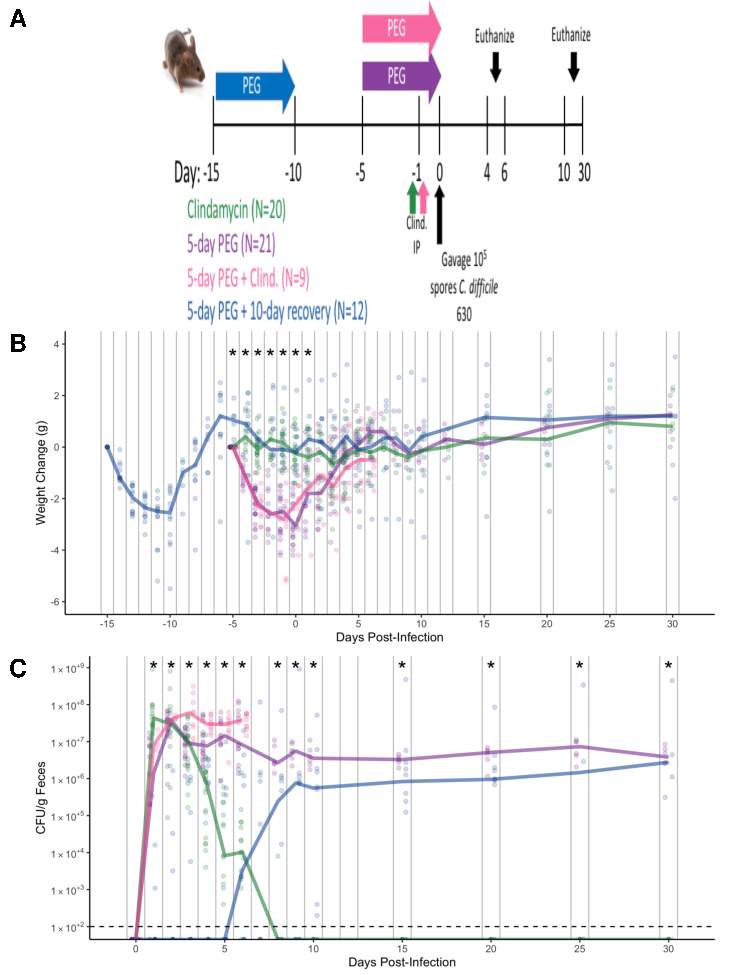
\includegraphics{figure_1.pdf}

\textbf{Figure 1. 5-day PEG treatment prolongs susceptibility and mice
become persistently colonized with \emph{C. difficile}.} A. Setup of the
experimental time line for experiments with 5-day PEG treated mice
consisting of 4 treatment groups. 1. Clindamycin was administered at 10
mg/kg by intraperitoneal injection. 2. 15\% PEG 3350 was administered in
the drinking water for five days. 3. 5-day PEG plus clindamycin
treatment. 4. 5-day PEG plus 10-day recovery treatment. All treatment
groups were then challenged with 10\textsuperscript{5} \emph{C.
difficile} 630 spores. A subset of mice were euthanized on either 4 or 6
days post-challenge and tissues were collected for histopathology
analysis, the remaining mice were followed through 20 or 30 days
post-challenge. B. Weight change from baseline weight in groups after
treatment with PEG and/or clindamycin, followed by \emph{C. difficile}
challenge. C. \emph{C. difficile} CFU/gram stool measured over time via
serial dilutions(N = 10-59 mice per time point). The black line
represents the limit of detection for the first serial dilution. CFU
quantification data was not available for each mouse due to stool
sampling difficulties (particularly the day the mice came off of the PEG
treatment) or early deaths. For B-C, lines represent the median for each
treatment group and circles represent samples from individual mice.
Asterisks indicate time points where the weight change or CFU/g was
significantly different (\emph{P} \textless{} 0.05) between groups by
the Kruskal-Wallis test with Benjamini-Hochberg correction for testing
multiple time points. The data presented are from a total of 5 separate
experiments. \newpage

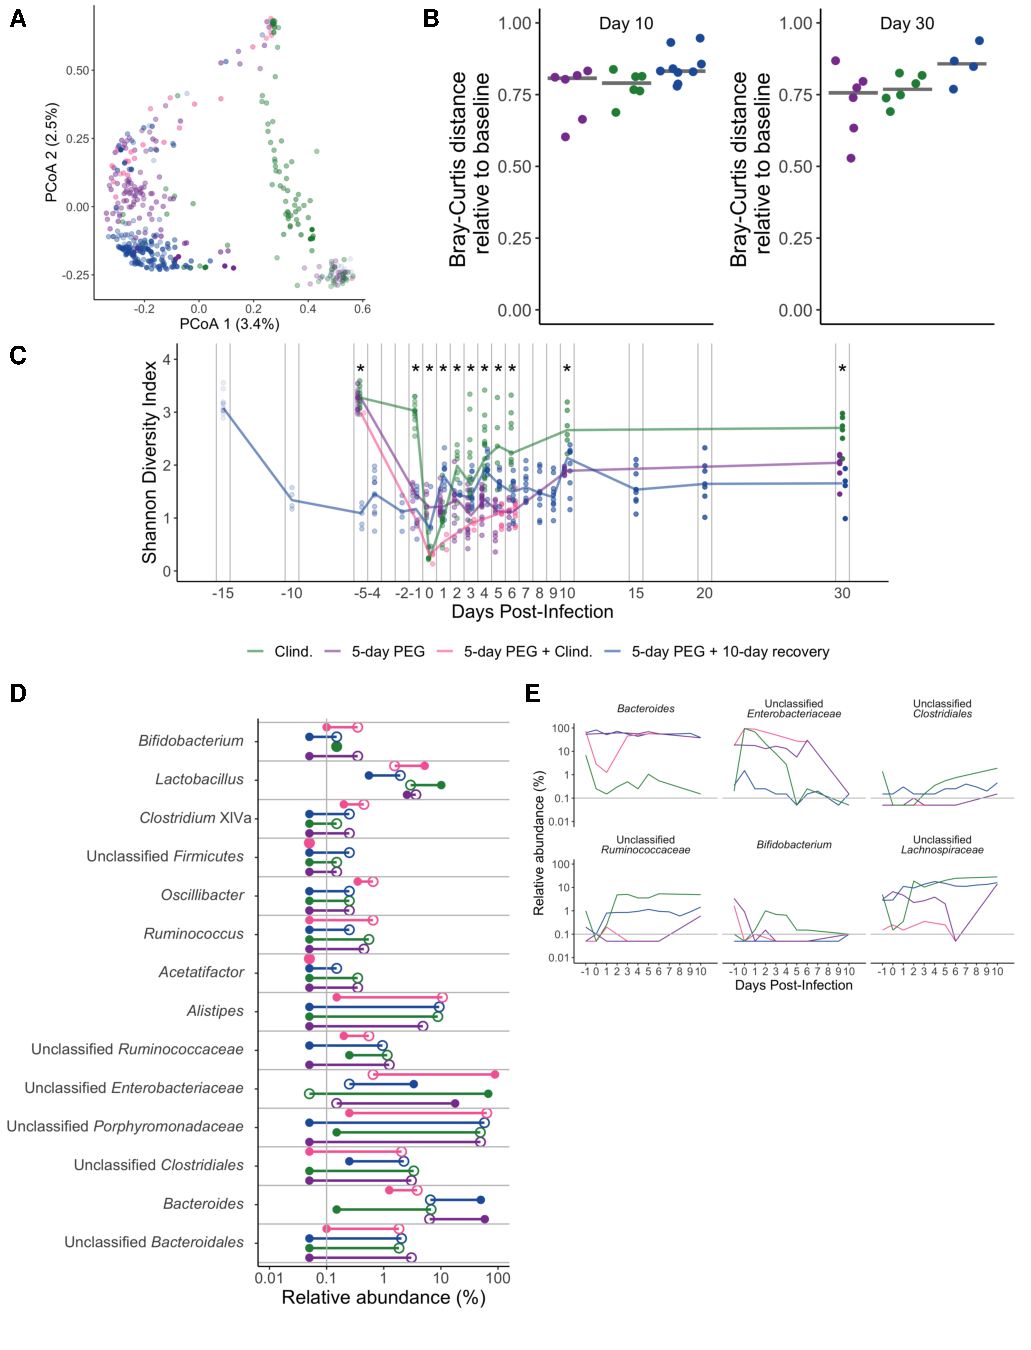
\includegraphics{figure_2.pdf} \textbf{Figure 2. 5-day PEG treatment
disrupts the stool microbiota for a longer amount of time compared to
clindamycin-treated mice.} A. Principal Coordinate analysis (PCoA) of
Bray-Curtis distances from stool samples collected throughout the
experiment. Each circle represents a sample from an individual mouse and
the transparency of the symbol corresponds to the day post-challenge.
See Data Set S1, sheet 1 for PERMANOVA results. B. Bray-Curtis distances
of stool samples collected on either day 10 or 30 post-challenge
relative to the baseline sample collected for each mouse (before any
drug treatments were administered). The symbols represent samples from
individual mice and the line indicates the median value for each
treatment group. C. Shannon diversity in stool communities over time.
The line indicates the median value for each treatment group (Data Set
S1, sheet 2). D. 14 of the 33 genera affected by PEG treatment (Data Set
S1, sheet 3). The symbols represent the median relative abundance for a
treatment group at either baseline (open circle) or 1-day post treatment
(closed circle). Relative abundance data from paired baseline and 1-day
post treatment stool sampes from the 5-day PEG and 5-day PEG plus 10-day
recovery groups were analyzed by paired Wilcoxan signed-rank test with
Benjamini-Hochberg correction for testing all identified genera. The
clindamycin and 5-day PEG plus clindamycin treatment groups are shown on
the plot for comparison. E. 6 of the 24 genera that were significantly
different between the treatment groups over multiple time points (see
Data Set S1, sheet 4 for complete list). The 5-day PEG plus clindamycin
treatment group was only followed through 6-days post-challenge.
Differences between treatment groups were identified by Kruskal-Wallis
test with Benjamini-Hochberg correction for testing all identified
genera (*, \emph{P} \textless{} 0.05). The gray vertical line (D) and
horizontal vertical lines (E) indicate the limit of detection. \newpage

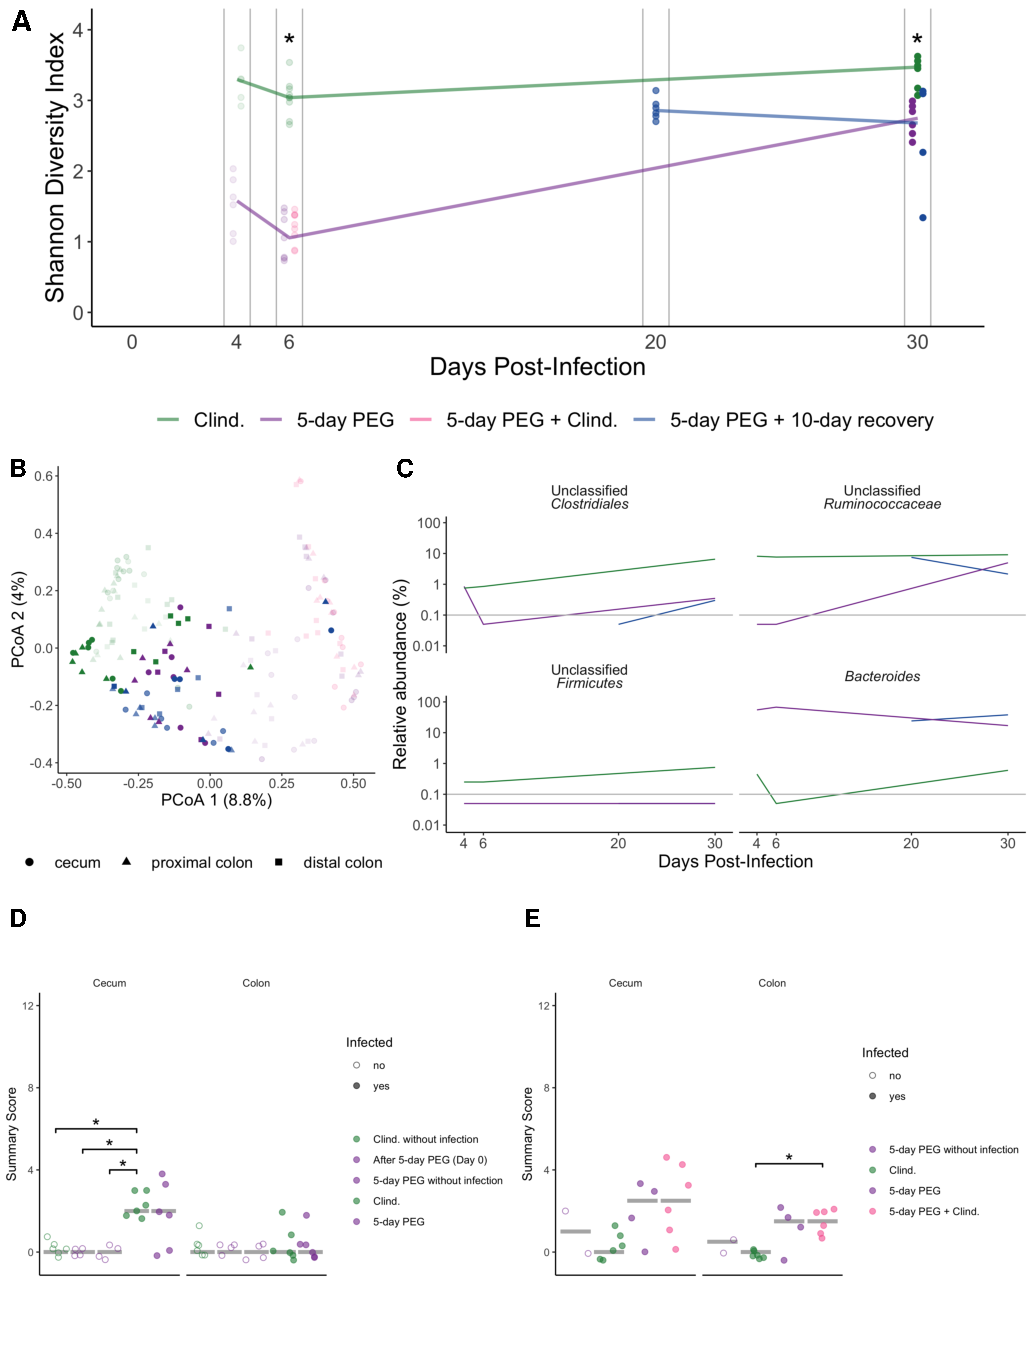
\includegraphics{figure_3.pdf} \textbf{Figure 3. 5-day PEG treatment
does not result in more severe CDIs, although mucosal microbiota is
altered.} A. Shannon diversity in cecum communities over time. The
colors of the symbols and lines represent individual and median relative
abundance values for four treatment groups (Data Set S1, sheet 6). B.
PCoA of Bray-Curtis distances from mucosal samples collected throughout
the experiment. Circles, triangles, and squares indicate the cecum,
proximal colon, and distal colon communities, respectively. Transparency
of the symbol corresponds to the day post-challenge that the sample was
collected. See Data Set S1, sheet 7 for PERMANOVA results. C. The median
relative abundance of the 4 genera that were significantly different
between the cecum communities of different treatment groups on day 6 and
day 30 post-challenge (Data Set S1, sheet 8). The gray vertical lines
indicate the limit of detection. D-E. The histopathology summary scores
from cecum and colon H\&E stained tissue sections. The summary score is
the total score based on evaluation of edema, cellular infiltration, and
inflammation in either the cecum or colon tissue. Each category is given
a score ranging from 0-4, thus the maximum possible summary score is 12.
The tissue for histology was collected at either 4 (D) or 6 (E) days
post-challenge with the exception that one set of 5-day PEG treated
mock-challenged mice were collected on day 0 post-challenge (first set
of open purple circles in D). Histology data were analyzed with the
Kruskal-Wallis test followed by pairwise Wilcoxon comparisons with
Benjamini-Hochberg correction. *, \emph{P} \textless{} 0.05. \newpage

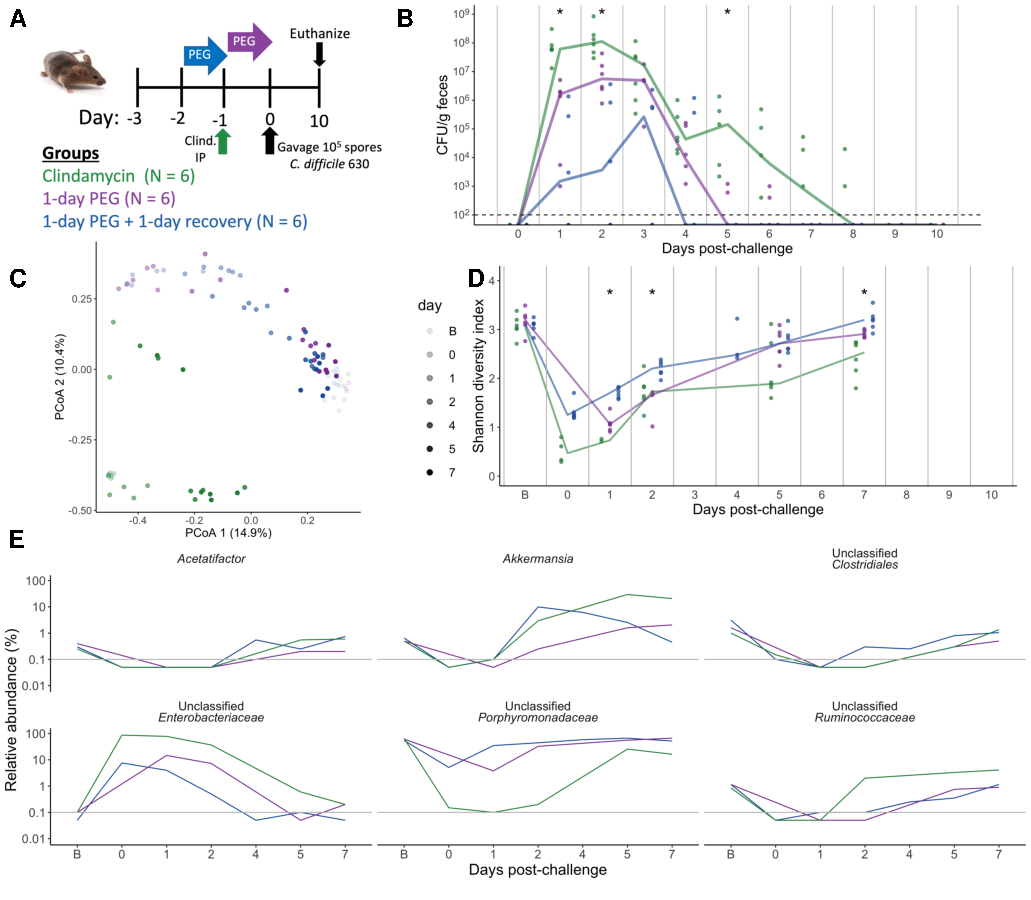
\includegraphics{figure_4.pdf} \textbf{Figure 4. 1-day PEG treatment
renders mice susceptible to transient \emph{C. difficile} colonization.}
A. Setup of the experimental time line for the 1-day PEG treated mice
consisting of 3 treatment groups. 1. Clindamycin was administered at 10
mg/kg by intraperitoneal injection. 2. 15\% PEG 3350 was administered in
the drinking water for 1 day. 3. 1-day PEG plus 1-day recovery. The
three treatment groups were then challenged with 10\textsuperscript{5}
\emph{C. difficile} 630 spores. B. \emph{C. difficile} CFU/gram stool
measured over time (N = 12-18 mice per time point) by serial dilutions.
The black dashed horizontal line represents the limit of detection for
the first serial dilution. For B and D, asterisks indicate time points
where there was a significant difference (\emph{P} \textless{} 0.05)
between treatment groups by Kruskall-Wallis test with Benjamini-Hochberg
correction for testing multiple time points. For B-D, each symbol
represents a sample from an individual mouse and lines indicate the
median value for each treatment group. C. PCoA of Bray-Curtis distances
from stool communities collected over time (day: R\textsuperscript{2} =
0.43; group: R\textsuperscript{2} = 0.19, Data Set S1, sheet 11). Symbol
transparency represents the day post-challenge of the experiment. For
C-E, the B on the day legend or days post-challenge X-axis stands for
baseline and represents the sample that was collected prior to any drug
treatments. D. Shannon diversity in stool communities over time (Data
Set S1, sheet 12). E. Median relative abundances per treatment group for
6 out of the 14 genera that were affected by treatment, but recovered
close to baseline levels by 7 days post-challenge (Fig. 3E, Data Set S1,
sheets 13 and 14). Paired stool sample relative abundance values either
baseline and day 1 or baseline and day 7 were analyzed by paired
Wilcoxan signed-rank test with Benjamini-Hochberg correction for testing
all identified genera. Only genera that were different between baseline
and 1-day post-challenge, but not baseline and 7-days post-challenge are
shown. The gray horizontal lines represents the limit of detection.

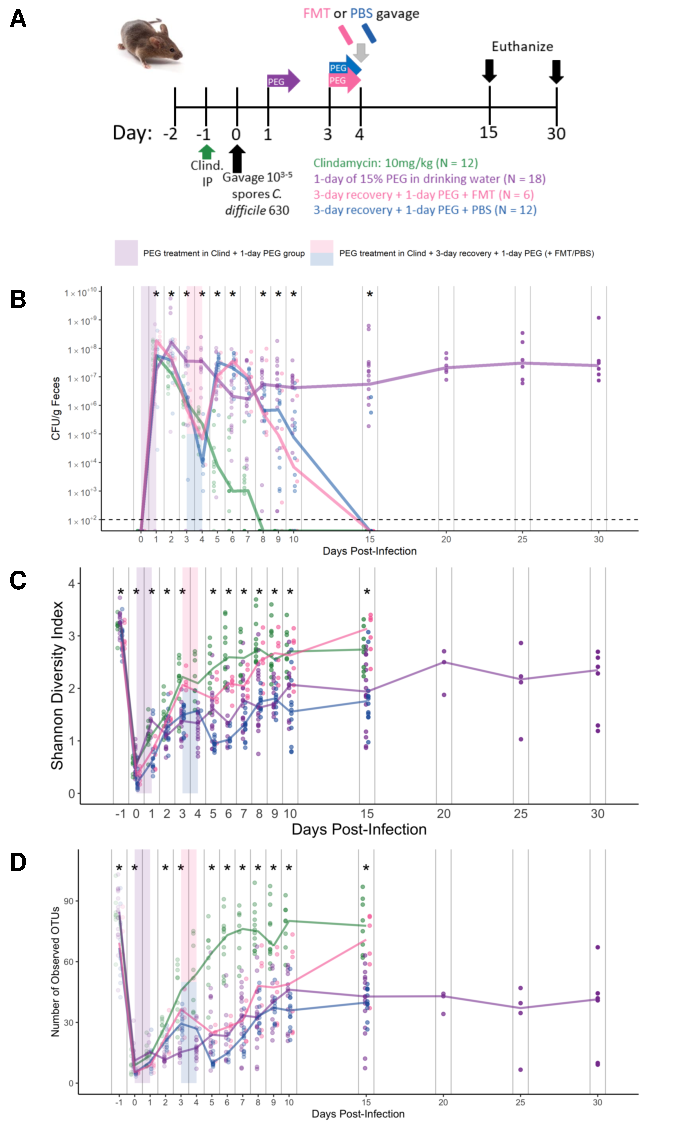
\includegraphics{figure_5.pdf} \textbf{Figure 5. 1-day PEG treatment
post \emph{C. difficile} challenge prolongs colonization regardless of
whether an FMT is also administered.} A. Setup of the experimental time
line for experiments with post-challenge PEG treated mice. There were a
total of 4 different treatment groups. All mice were administered 10
mg/kg clindamycin intraperitoneally (IP) 1 day before challenge with
10\textsuperscript{3-5} \emph{C. difficile} 630 spores. 1. Received no
additional treatment (Clindamycin). 2. Immediately after \emph{C.
difficile} challenge, mice received 15\% PEG 3350 in the drinking water
for 1 day. 3-4. 3-days after challenge, mice received 1-day PEG
treatment and then received either 100 microliters a fecal microbiota
transplant (3) or PBS (4) solution by oral gavage. Mice were followed
through 15-30 days post-challenge (only the post-CDI 1-day PEG group was
followed through 30 days post-challenge). B. CFU/g of \emph{C.
difficile} stool measured over time via serial dilutions. The black line
represents the limit of detection for the first serial dilution. C-D.
Shannon diversity (C) and richness (D) in stool communities over time
(Data Set S1, sheets 15 and 16). B-D. Each symbol represents a stool
sample from an individual mouse with the lines representing the median
value for each treatment group. Asterisks indicate time points with
significant differences (\emph{P} \textless{} 0.05) between groups by
the Kruskall-Wallis test with a Benjamini-Hochberg correction for
testing multiple times points. Colored rectangles indicates the 1-day
PEG treatment period for applicable groups. The data presented are from
a total of 3 separate experiments. \newpage

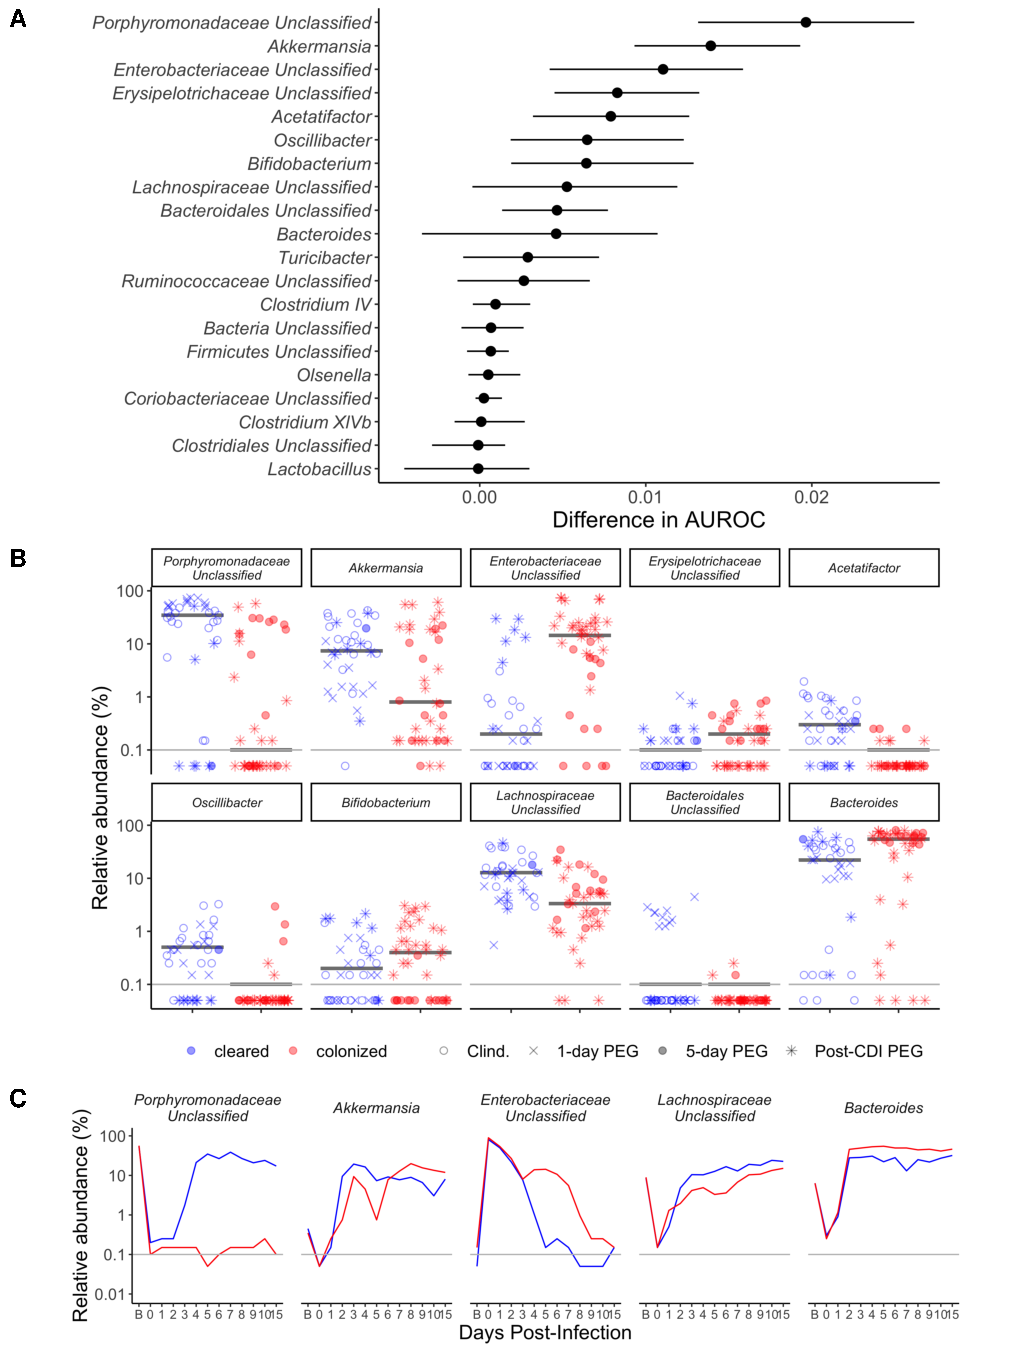
\includegraphics{figure_6.pdf} \textbf{Figure 6. For 1-day PEG treatment
post \emph{C. difficile} challenge mice that also receive an FMT only
some bacterial genera were restored.} A. PCoA of Bray-Curtis distances
from stool samples collected over time as well as the FMT solution that
was administered to one of the treatment groups. Each circle represents
an individual sample, the transparency of the circle corresponds to day
post-challenge. See Data Set S1, sheet 17 for PERMANOVA results. B.
Median relative abundances of 2 genera that were significantly different
over multiple time points in mice that were administered either FMT or
PBS solution via gavage C. Median relative abundances of the top 6 out
of 24 genera that were significant over multiple time points, plotted
over time (see Data Set S1, sheet 18 for complete list). For B-C,
colored rectangles indicates the 1-day PEG treatment period for
applicable groups. Gray horizontal lines represent the limit of
detection. Differences between treatment groups were identified by
Kruskal-Wallis test with Benjamini-Hochberg correction for testing all
identified genera. For pairwise comparisons of the groups (B), we
performed pairwise Wilcoxon comparisons with Benjamini-Hochberg
correction for testing all combinations of group pairs.

\newpage

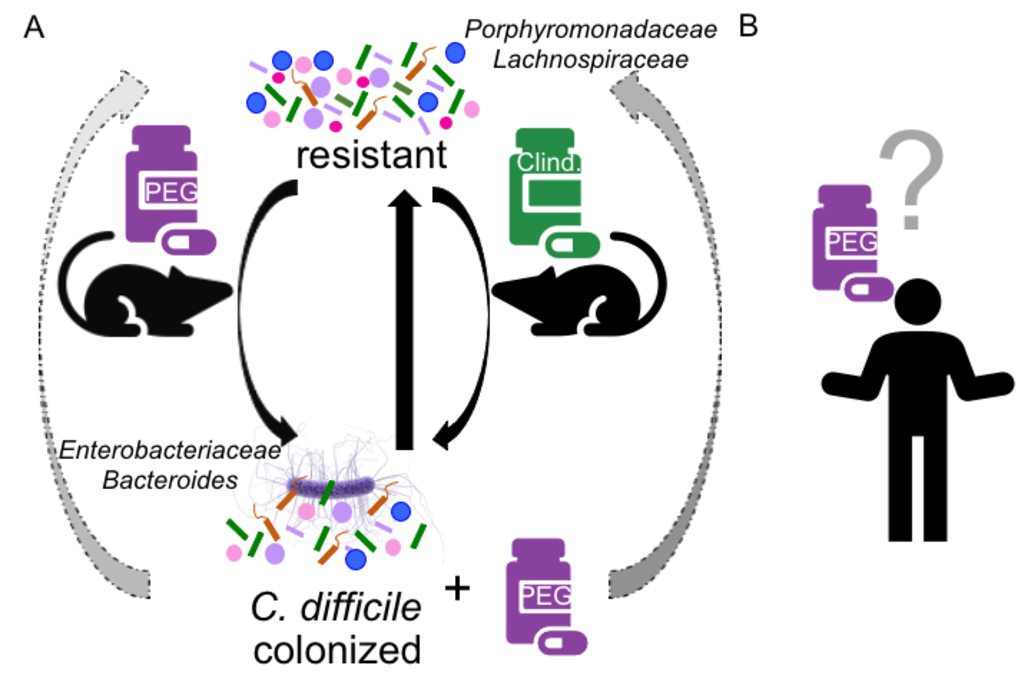
\includegraphics{figure_7.pdf} \textbf{Figure 7. Specific microbiota
features associated with prolonged \emph{C. difficile} colonization in
PEG treated mice.} A. Top ten bacteria that contributed to the random
forest model trained on 5-day post-challenge community relative
abundance data, predicting whether mice would still be colonized with
\emph{C. difficile} 10 days post-challenge. The median (point) and
interquartile range (lines) change in AUROC when the bacteria were left
out of the model by permutation feature importance analysis. B. The
median relative abundances of the top ten bacteria that contributed to
the random forest classification model at 5 days post-challenge . Red
indicates the mice were still colonized with \emph{C. difficile} while
blue indicates mice that cleared \emph{C. difficile} 10 days
post-challenge and the black horizontal line represents the median
relative abundance for the two categories. Each symbol represents a
stool sample from an individual mouse and the shape of the symbol
indicates whether the PEG-treated mice received a 5-day (Fig. 1-3),
1-day (Fig. 4) or post-challenge PEG (Fig. 5-6) treatment. C. The median
relative abundances of the 5 genera with greater than 1\% median
relative abundance in the stool community over time. For B-C, the gray
horizontal lines represents the limit of detection. \newpage

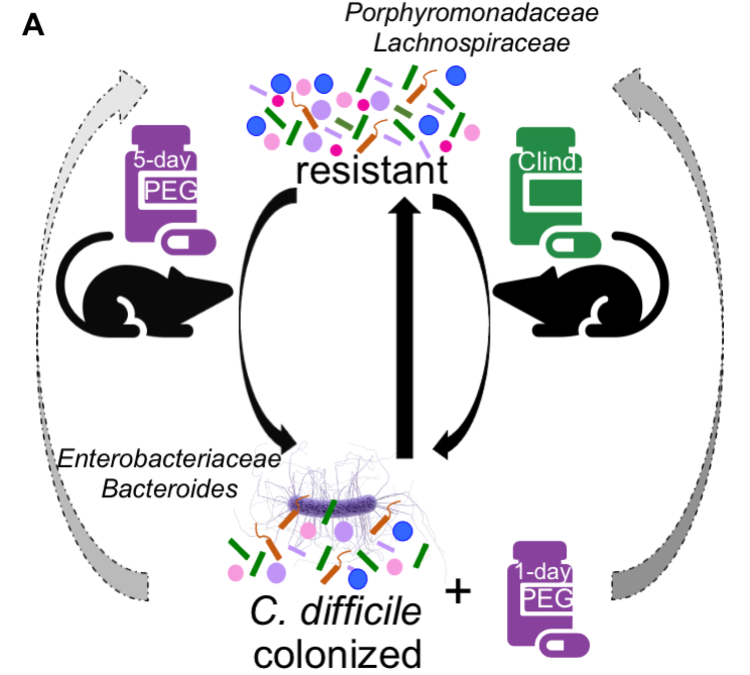
\includegraphics{figure_8.pdf}

\textbf{Figure 8. Schematic summarizing findings.} The gut microbiota of
our C57Bl/6 mice is resistant to \emph{C. difficle} but treatment with
either the antibiotic, clindamycin, or the osmotic laxative, PEG 3350,
renders the mice susceptible to \emph{C. difficile} colonization.
Recovery of colonization resistance in clindamycin-treated mice is
relatively straightforward and the mice clear \emph{C.difficile} within
10 days post-challenge. However, for mice that received either a 5-day
PEG treatment prior to \emph{C. difficile} challenge or a 1-day PEG
treatment post-challenge recovery of colonization resistance was delayed
because most mice were still colonized with \emph{C. difficile} 10 days
post-challenge. We found increased relative abundances of
\emph{Porphyromonadaceae} and \emph{Lachnospiraceae} were associated
with recovery of colonization resistance, while increased relative
abundances of \emph{Enterobacteriaceae} and \emph{Bacteroides} were
associated with prolonged \emph{C. difficle} colonization. \newpage

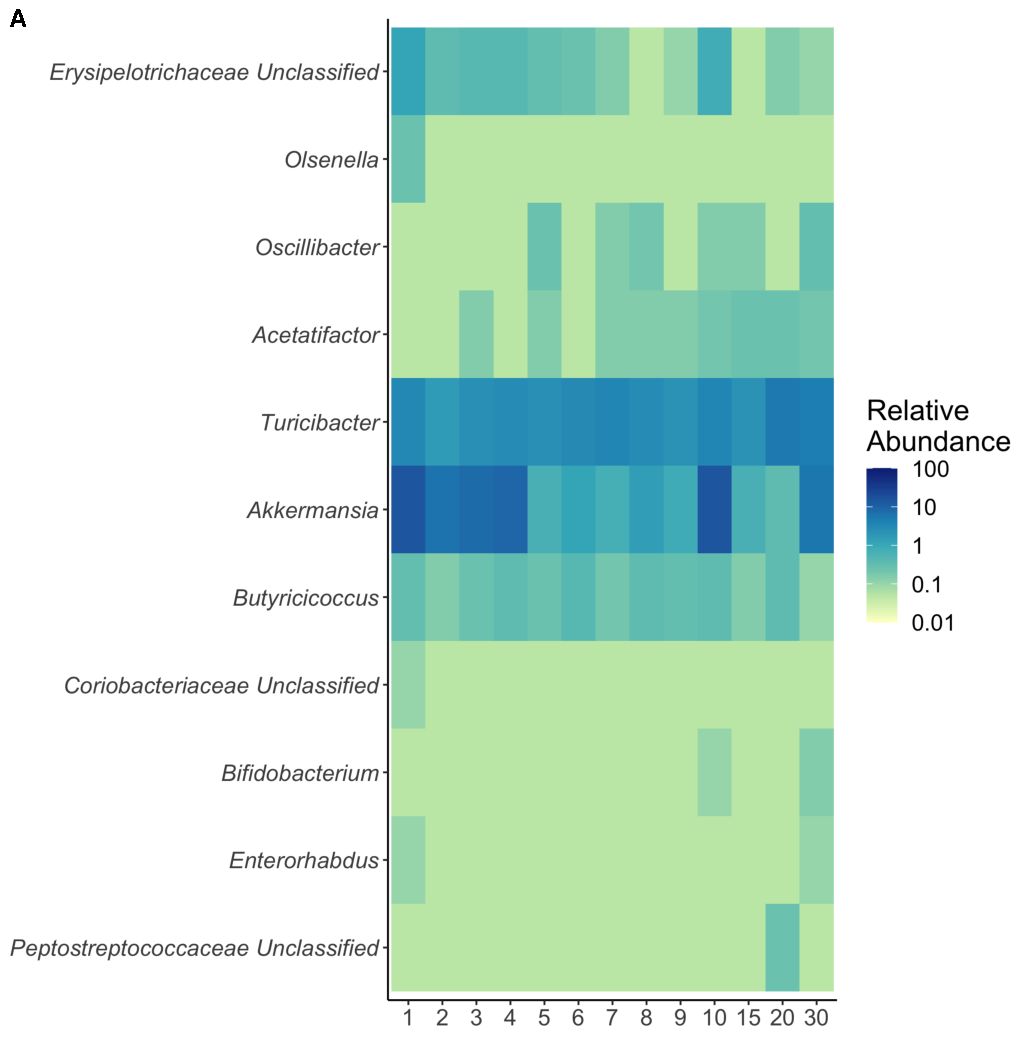
\includegraphics{figure_S1.pdf} \textbf{Figure S1. Microbiota dynamics
post-challenge in the 5-day PEG treatment plus 10-day recovery mice.} A.
\emph{C. difficile} CFU/g over time in the stool samples collected from
5-day PEG treated mice that were allowed to recover for 10 days prior to
challenge. Same data presented in Fig. 1C, but the data for the other 3
treatment groups have been removed and each line represents the CFU over
time for an individual mouse. Mouse 10 was found dead 6 days
post-challenge. B. Relative abundances of eight bacterial genera from
day 0 post-challenge onward in each of the 10-day recovery mice. We
analyzed samples from day 0 and day 8 post-challenge, which represented
the time points where mice were challenged with \emph{C. difficile} and
when the median relative \emph{C. difficile} CFU stabilized for the
group using the paired Wilcoxan signed-rank test, but no genera were
significantly different after Benjamini-Hochberg correction (Data Set
S1, sheet 5). \newpage

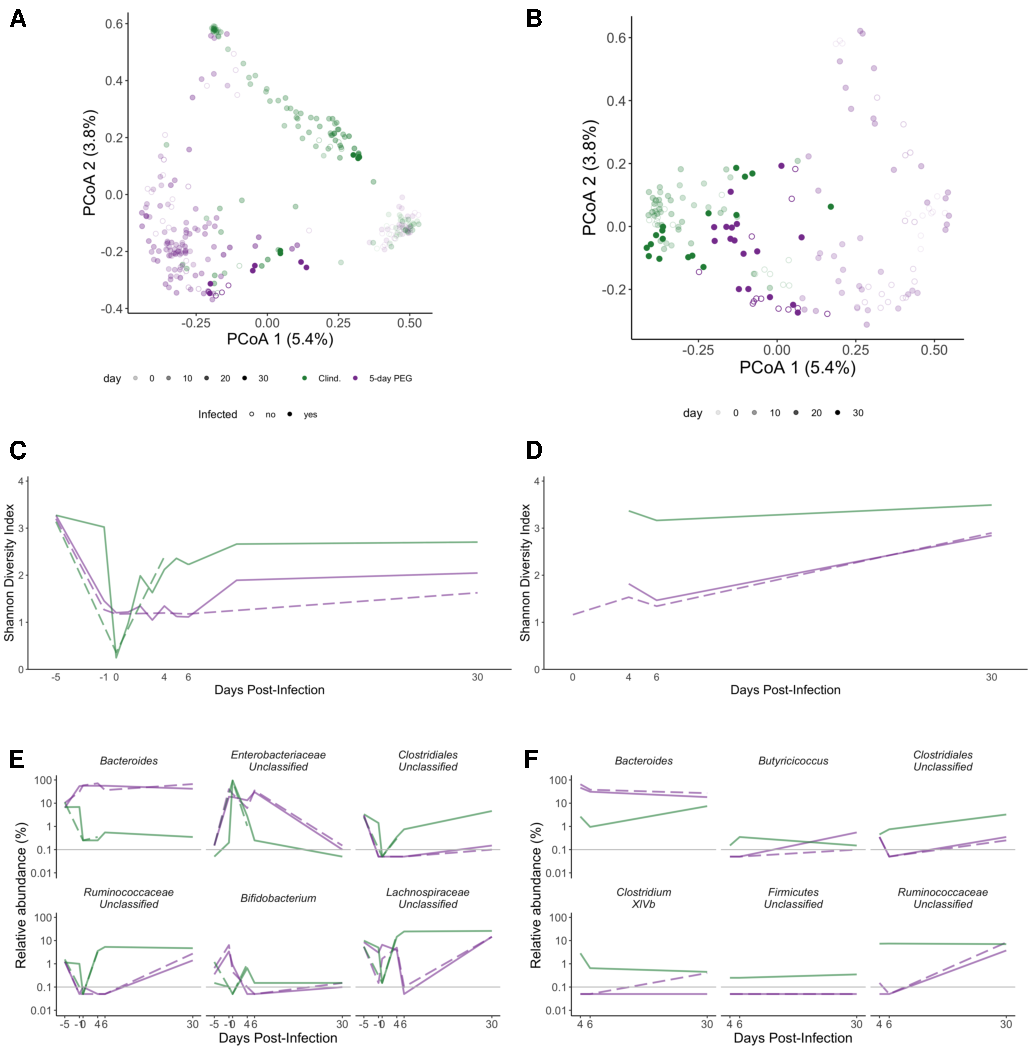
\includegraphics{figure_S2.pdf} \textbf{Figure S2. PEG treatment still
has a large impact on the mucosal microbiota 6 days post-challenge} A.
The relative abundances of the 10 bacterial genera that were
significantly different between treatment groups at 6 days
post-infection in the cecum tissue (the relative abundances of the 10
genera were also significantly different in the proximal and distal
colon tissues, Data Set S1, sheets 8, 9, and 10). Each symbol represents
a tissue sample from an individual mouse, the black horizontal lines
represents the median relative abundances for each treatment group. B.
The relative abundance of \emph{Peptostreptococacceae} in the three
types of tissue sample communities over time. For A-B, the gray
horizontal lines represent the limit of detection. \newpage

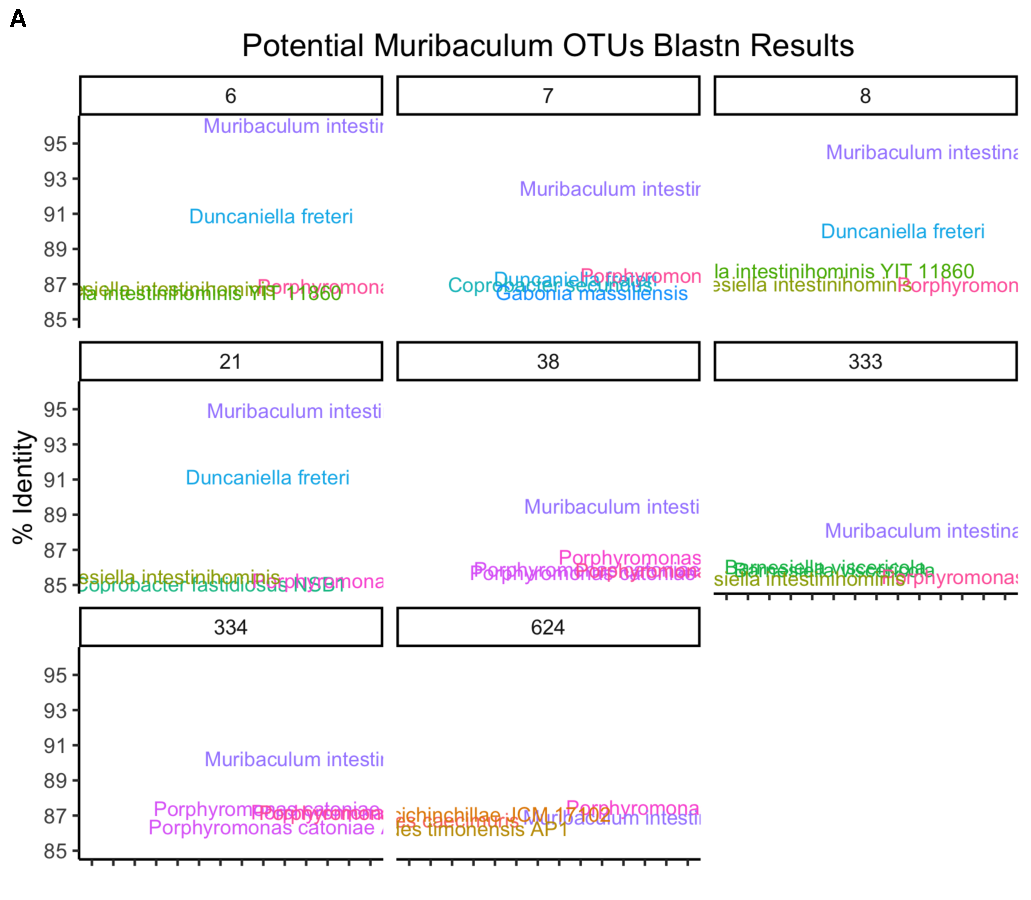
\includegraphics{figure_S3.pdf} \textbf{Figure S3. \emph{C. difficile}
challenge does not enhance the disruptive effect of PEG on the
microbiota.} A, D. PCoAs of the Bray-Curtis distances from the stool (A)
and tissue (D) communities from mock- and \emph{C. difficile}-challenged
treatment groups. Each symbol represents a sample from an individual
mouse with open and closed circles representing mock and \emph{C.
difficile}-challenged mice, respectively. B, E. Median Shannon diversity
in stool (B) and tissue (E) communities collected over time. C, F. The
median relative abundances of genera that were significantly different
between the \emph{C. difficile} challenged treatment groups in either
the stool (Fig. 2E) or cecum tissue (Fig. 3C) communities in the stool
(C) and tissue (F) communities from mock- and \emph{C.
difficile}-challenged mice. For B-F, the dashed and solid lines
represent the median value for mock and \emph{C. difficile}-challenged
mice, respectively. For E-F, tissues from mock-challenged clindamycin
treated mice were only collected 4 days post-challenge so there is no
dashed line for this group. \newpage

\hypertarget{data-set-s1}{%
\subsection{Data Set S1}\label{data-set-s1}}

\textbf{Data Set S1, Sheets 1-19. Excel workbook with 19 sheets.}

\textbf{Data Set S1, Sheet 1. PERMANOVA results for the stool
communities from mice in the 5-day PEG subset.}

\textbf{Data Set S1, Sheet 2. Shannon diversity analysis for the stool
communities from mice in the 5-day PEG subset.}

\textbf{Data Set S1, Sheet 3. Genera with relative abundances impacted
by PEG treatment based on stool communities of 5-day PEG treated mice.}

\textbf{Data Set S1, Sheet 4. Genera with relative abundances that vary
between treatment groups in the stool communities from mice in the 5-day
PEG subset.}

\textbf{Data Set S1, Sheet 5. Statistical analysis results for genera
with relative abundances that varied in stool communities in the 5-day
PEG plus 10-day recovery mice between the day 1 and day 8 time points.}

\textbf{Data Set S1, Sheet 6. Shannon diversity analysis for the cecum
communities from mice in the 5-day PEG experiments.}

\textbf{Data Set S1, Sheet 7. PERMANOVA results for the tissue
communities from mice in the 5-day PEG subset.}

\textbf{Data Set S1, Sheet 8. Genera with relative abundances that vary
between treatment groups in the cecum communities from mice in the 5-day
PEG esubset.}

\textbf{Data Set S1, Sheet 9. Genera with relative abundances that vary
between treatment groups in the proximal colon communities from mice in
the 5-day PEG subset.}

\textbf{Data Set S1, Sheet 10. Genera with relative abundances that vary
between treatment groups in the distal colon communities from mice in
the set of 5-day PEG subset.}

\textbf{Data Set S1, Sheet 11. PERMANOVA results for the stool
communities from mice in the set of 1-day PEG subset.}

\textbf{Data Set S1, Sheet 12. Shannon diversity analysis for the stool
communities from mice in the 1-day PEG experiments.}

\textbf{Data Set S1, Sheet 13. Genera with different relative abundances
between the baseline and day 1 time points in the 1-day PEG subset.}

\textbf{Data Set S1, Sheet 14. Genera with different relative abundances
between the baseline and day 7 time points in the 1-day PEG subset..}

\textbf{Data Set S1, Sheet 15. Shannon diversity analysis for the stool
communities from mice in the post-challenge PEG experiments.}

\textbf{Data Set S1, Sheet 16. Richness analysis for the stool
communities from mice in the post-challenge PEG experiments.}

\textbf{Data Set S1, Sheet 17. PERMANOVA results for the stool
communities from mice in the post-challenge PEG subset.}

\textbf{Data Set S1, Sheet 18. Genera with relative abundances that vary
between treatment groups in the stool communities from mice in the
post-challenge PEG subset.}

\textbf{Data Set S1, Sheet 19. AUROC results for the 100 different seeds
from each of the 3 models tested.}

\end{document}
